% Options for packages loaded elsewhere
\PassOptionsToPackage{unicode}{hyperref}
\PassOptionsToPackage{hyphens}{url}
%
\documentclass[
]{book}
\usepackage{lmodern}
\usepackage{amssymb,amsmath}
\usepackage{ifxetex,ifluatex}
\ifnum 0\ifxetex 1\fi\ifluatex 1\fi=0 % if pdftex
  \usepackage[T1]{fontenc}
  \usepackage[utf8]{inputenc}
  \usepackage{textcomp} % provide euro and other symbols
\else % if luatex or xetex
  \usepackage{unicode-math}
  \defaultfontfeatures{Scale=MatchLowercase}
  \defaultfontfeatures[\rmfamily]{Ligatures=TeX,Scale=1}
\fi
% Use upquote if available, for straight quotes in verbatim environments
\IfFileExists{upquote.sty}{\usepackage{upquote}}{}
\IfFileExists{microtype.sty}{% use microtype if available
  \usepackage[]{microtype}
  \UseMicrotypeSet[protrusion]{basicmath} % disable protrusion for tt fonts
}{}
\makeatletter
\@ifundefined{KOMAClassName}{% if non-KOMA class
  \IfFileExists{parskip.sty}{%
    \usepackage{parskip}
  }{% else
    \setlength{\parindent}{0pt}
    \setlength{\parskip}{6pt plus 2pt minus 1pt}}
}{% if KOMA class
  \KOMAoptions{parskip=half}}
\makeatother
\usepackage{xcolor}
\IfFileExists{xurl.sty}{\usepackage{xurl}}{} % add URL line breaks if available
\IfFileExists{bookmark.sty}{\usepackage{bookmark}}{\usepackage{hyperref}}
\hypersetup{
  pdftitle={An Introduction to Probability and Simulation},
  pdfauthor={Kevin Ross},
  hidelinks,
  pdfcreator={LaTeX via pandoc}}
\urlstyle{same} % disable monospaced font for URLs
\usepackage{color}
\usepackage{fancyvrb}
\newcommand{\VerbBar}{|}
\newcommand{\VERB}{\Verb[commandchars=\\\{\}]}
\DefineVerbatimEnvironment{Highlighting}{Verbatim}{commandchars=\\\{\}}
% Add ',fontsize=\small' for more characters per line
\usepackage{framed}
\definecolor{shadecolor}{RGB}{248,248,248}
\newenvironment{Shaded}{\begin{snugshade}}{\end{snugshade}}
\newcommand{\AlertTok}[1]{\textcolor[rgb]{0.94,0.16,0.16}{#1}}
\newcommand{\AnnotationTok}[1]{\textcolor[rgb]{0.56,0.35,0.01}{\textbf{\textit{#1}}}}
\newcommand{\AttributeTok}[1]{\textcolor[rgb]{0.77,0.63,0.00}{#1}}
\newcommand{\BaseNTok}[1]{\textcolor[rgb]{0.00,0.00,0.81}{#1}}
\newcommand{\BuiltInTok}[1]{#1}
\newcommand{\CharTok}[1]{\textcolor[rgb]{0.31,0.60,0.02}{#1}}
\newcommand{\CommentTok}[1]{\textcolor[rgb]{0.56,0.35,0.01}{\textit{#1}}}
\newcommand{\CommentVarTok}[1]{\textcolor[rgb]{0.56,0.35,0.01}{\textbf{\textit{#1}}}}
\newcommand{\ConstantTok}[1]{\textcolor[rgb]{0.00,0.00,0.00}{#1}}
\newcommand{\ControlFlowTok}[1]{\textcolor[rgb]{0.13,0.29,0.53}{\textbf{#1}}}
\newcommand{\DataTypeTok}[1]{\textcolor[rgb]{0.13,0.29,0.53}{#1}}
\newcommand{\DecValTok}[1]{\textcolor[rgb]{0.00,0.00,0.81}{#1}}
\newcommand{\DocumentationTok}[1]{\textcolor[rgb]{0.56,0.35,0.01}{\textbf{\textit{#1}}}}
\newcommand{\ErrorTok}[1]{\textcolor[rgb]{0.64,0.00,0.00}{\textbf{#1}}}
\newcommand{\ExtensionTok}[1]{#1}
\newcommand{\FloatTok}[1]{\textcolor[rgb]{0.00,0.00,0.81}{#1}}
\newcommand{\FunctionTok}[1]{\textcolor[rgb]{0.00,0.00,0.00}{#1}}
\newcommand{\ImportTok}[1]{#1}
\newcommand{\InformationTok}[1]{\textcolor[rgb]{0.56,0.35,0.01}{\textbf{\textit{#1}}}}
\newcommand{\KeywordTok}[1]{\textcolor[rgb]{0.13,0.29,0.53}{\textbf{#1}}}
\newcommand{\NormalTok}[1]{#1}
\newcommand{\OperatorTok}[1]{\textcolor[rgb]{0.81,0.36,0.00}{\textbf{#1}}}
\newcommand{\OtherTok}[1]{\textcolor[rgb]{0.56,0.35,0.01}{#1}}
\newcommand{\PreprocessorTok}[1]{\textcolor[rgb]{0.56,0.35,0.01}{\textit{#1}}}
\newcommand{\RegionMarkerTok}[1]{#1}
\newcommand{\SpecialCharTok}[1]{\textcolor[rgb]{0.00,0.00,0.00}{#1}}
\newcommand{\SpecialStringTok}[1]{\textcolor[rgb]{0.31,0.60,0.02}{#1}}
\newcommand{\StringTok}[1]{\textcolor[rgb]{0.31,0.60,0.02}{#1}}
\newcommand{\VariableTok}[1]{\textcolor[rgb]{0.00,0.00,0.00}{#1}}
\newcommand{\VerbatimStringTok}[1]{\textcolor[rgb]{0.31,0.60,0.02}{#1}}
\newcommand{\WarningTok}[1]{\textcolor[rgb]{0.56,0.35,0.01}{\textbf{\textit{#1}}}}
\usepackage{longtable,booktabs}
% Correct order of tables after \paragraph or \subparagraph
\usepackage{etoolbox}
\makeatletter
\patchcmd\longtable{\par}{\if@noskipsec\mbox{}\fi\par}{}{}
\makeatother
% Allow footnotes in longtable head/foot
\IfFileExists{footnotehyper.sty}{\usepackage{footnotehyper}}{\usepackage{footnote}}
\makesavenoteenv{longtable}
\usepackage{graphicx}
\makeatletter
\def\maxwidth{\ifdim\Gin@nat@width>\linewidth\linewidth\else\Gin@nat@width\fi}
\def\maxheight{\ifdim\Gin@nat@height>\textheight\textheight\else\Gin@nat@height\fi}
\makeatother
% Scale images if necessary, so that they will not overflow the page
% margins by default, and it is still possible to overwrite the defaults
% using explicit options in \includegraphics[width, height, ...]{}
\setkeys{Gin}{width=\maxwidth,height=\maxheight,keepaspectratio}
% Set default figure placement to htbp
\makeatletter
\def\fps@figure{htbp}
\makeatother
\setlength{\emergencystretch}{3em} % prevent overfull lines
\providecommand{\tightlist}{%
  \setlength{\itemsep}{0pt}\setlength{\parskip}{0pt}}
\setcounter{secnumdepth}{5}
\usepackage{booktabs}
\usepackage{amsthm}
\makeatletter
\def\thm@space@setup{%
  \thm@preskip=8pt plus 2pt minus 4pt
  \thm@postskip=\thm@preskip
}
\makeatother
\usepackage[]{natbib}
\bibliographystyle{apalike}

\title{An Introduction to Probability and Simulation}
\author{Kevin Ross}
\date{2020-07-11}

\usepackage{amsthm}
\newtheorem{theorem}{Theorem}[chapter]
\newtheorem{lemma}{Lemma}[chapter]
\newtheorem{corollary}{Corollary}[chapter]
\newtheorem{proposition}{Proposition}[chapter]
\newtheorem{conjecture}{Conjecture}[chapter]
\theoremstyle{definition}
\newtheorem{definition}{Definition}[chapter]
\theoremstyle{definition}
\newtheorem{example}{Example}[chapter]
\theoremstyle{definition}
\newtheorem{exercise}{Exercise}[chapter]
\theoremstyle{remark}
\newtheorem*{remark}{Remark}
\newtheorem*{solution}{Solution}
\begin{document}
\maketitle

{
\setcounter{tocdepth}{1}
\tableofcontents
}
\hypertarget{preface}{%
\chapter*{Preface}\label{preface}}
\addcontentsline{toc}{chapter}{Preface}

\newcommand{\IP}{\textrm{P}}
\newcommand{\IQ}{\textrm{Q}}
\newcommand{\E}{\textrm{E}}
\newcommand{\Var}{\textrm{Var}}
\newcommand{\SD}{\textrm{SD}}
\newcommand{\Cov}{\textrm{Cov}}
\newcommand{\Corr}{\textrm{Corr}}
\newcommand{\Xbar}{\bar{X}}
\newcommand{\Ybar}{\bar{X}}
\newcommand{\xbar}{\bar{x}}
\newcommand{\ybar}{\bar{y}}
\newcommand{\ind}{\textrm{I}}
\newcommand{\dd}{\text{DDWDDD}}
\newcommand{\ep}{\epsilon}
\newcommand{\reals}{\mathbb{R}}



\hypertarget{why-study-probability-and-simulation}{%
\subsection*{\texorpdfstring{Why study probability \emph{and simulation}?}{Why study probability and simulation?}}\label{why-study-probability-and-simulation}}
\addcontentsline{toc}{subsection}{Why study probability \emph{and simulation}?}

Why study probability?

\begin{itemize}
\tightlist
\item
  Probability is the study of uncertainty, and life is uncertain
\item
  Probability is used in a wide variety of fields, including: \href{https://fivethirtyeight.com/features/not-even-scientists-can-easily-explain-p-values/}{statistics}, \href{https://www.ucdavis.edu/news/does-probability-come-quantum-physics/}{physics}, \href{https://en.wikipedia.org/wiki/Signal_processing}{engineering}, \href{https://www.ncbi.nlm.nih.gov/pmc/articles/PMC3843941/}{biology}, \href{https://cvi.asm.org/content/cdli/23/4/249.full.pdf}{medicine}, \href{https://www.marketwatch.com/story/the-4-called-the-last-financial-crisis-heres-what-they-see-causing-the-next-one-2018-09-13}{finance}, \href{https://www.ssa.gov/oact/STATS/table4c6.html}{actuarial science}, \href{https://projects.fivethirtyeight.com/2016-election-forecast/}{political science}, \href{https://en.wikipedia.org/wiki/Prosecutor\%27s_fallacy}{law}, \href{https://www.numberfire.com/nfl/lists/18685/the-10-biggest-plays-of-super-bowl-lii}{sports} , \ldots{}
\item
  Many topics and problems in probability are frequently misunderstood and sometimes counter intuitive, so it's worthwhile to take a careful study
\item
  ``Probabilistic thinking'' is an important component of statistical literacy (e.g.~how to assess risk when making decisions)
\item
  Probability provides the foundation for many important statistical concepts and methods such as p-values and confidence intervals
\end{itemize}

Why use \textbf{simulation} to study probability?

\begin{itemize}
\tightlist
\item
  Many concepts encountered in probability can seem esoteric; simulation helps make them more concrete.
\item
  Simulation provides an effective tool for analyzing probability models and for exploring effects of changing assumptions
\item
  Simulation can be used to check analytical solutions
\item
  Simulation is often the best or only method for investigating many problems which are too complex to solve analytically
\item
  Simulation-based reasoning is an important component of statistical literacy (e.g.~understanding a p-value via simulation)
\item
  Many statistical procedures employ simulation-based methods (e.g.~bootstrapping)
\end{itemize}

\hypertarget{learning-objectivesgoalsstyle-better-title}{%
\subsection{Learning Objectives/Goals/Style??? (Better title)}\label{learning-objectivesgoalsstyle-better-title}}

\begin{itemize}
\tightlist
\item
  Don't skimp on rigorous definitions (RV is function defined on probspace) but deemphasize mathematical computation (counting and calculus)
\item
  Emphasize simulation
\item
  Visualize in lots of plots
\item
  Start multivariate relationships early
\item
  Rely on statistical literacy
\item
  Active learning, workbook style
\end{itemize}

\hypertarget{symbulate}{%
\subsection*{Symbulate}\label{symbulate}}
\addcontentsline{toc}{subsection}{Symbulate}

This book uses the Python package Symbulate
(\url{https://github.com/dlsun/symbulate}) which provides a user friendly framework for conducting simulations involving probability models. The
syntax of Symbulate reflects the ``language of probability'' and makes it
intuitive to specify, run, analyze, and visualize the results of a
simulation. In Symbulate, probability spaces, events, random variables, and random processes are symbolic objects which can be manipulated, independently of their simulated realizations. Symbulate's consistency with the mathematics of
probability reinforces understanding of probabilistic concepts. The article \citet{symbulateJSE} discusses Symbulate and its features in more detail.

To install Symbulate, it is recommended that you first install the \href{https://www.anaconda.com/distribution/}{Anaconda distribution}, which is a Python environment with many scientific packages installed (including all of the packages that Symbulate is built on). After installing Anaconda, the recommended way to installing Symbulate is run the command

\begin{verbatim}
!pip install symbulate
\end{verbatim}

from inside a notebook. (The Symbulate package can also be downloaded and installed manually from the \href{/href\%7Bhttps://github.com/dlsun/symbulate\%7D}{Symbulate Github repository} following these \href{https://web.calpoly.edu/~dsun09/python.html}{instructions}.)

The following command imports Symbulate during a Python session.

\begin{Shaded}
\begin{Highlighting}[]
\ImportTok{from}\NormalTok{ symbulate }\ImportTok{import} \OperatorTok{*}
\end{Highlighting}
\end{Shaded}

The Symbulate command \texttt{plot()} produces graphics. These graphics can be customized (by changing axis limits, adding titles, legends, etc) using Matplotlib, and in particular the \texttt{pyplot} method, which can be imported with

\begin{verbatim}
import matplotlib
import matplotlib.pyplot as plt
\end{verbatim}

\href{http://jupyter.org/}{Jupyter} or \href{https://colab.research.google.com/notebooks/intro.ipynb\#}{Google Colab} notebooks provide a natural interface for Symbulate. The code in this book matches as closely as possible the commands that would be entered into cells in a notebook. However, certain commands that appear throughout the book are needed only to properly produce the output in this book, and not if working directly in notebooks. In particular, \texttt{plt.figure()} and \texttt{plt.show()} are not needed to produce graphics in Jupyter (with the use of the \texttt{\%matplotlib\ inline} ``magic''). In addition, Jupyter automatically displays the result of the last line in a cell; \texttt{print()} is generally not needed to display output (unless you wish to format it, or it is not the last line in the cell).

For example, a code snippet that appears in this book as

\begin{Shaded}
\begin{Highlighting}[]
\NormalTok{x }\OperatorTok{=}\NormalTok{ RV(Binomial(}\DecValTok{4}\NormalTok{, }\FloatTok{0.5}\NormalTok{)).sim(}\DecValTok{10000}\NormalTok{)}
\NormalTok{plt.figure()}
\NormalTok{x.plot()}
\NormalTok{plt.show()}
\BuiltInTok{print}\NormalTok{(x)}
\end{Highlighting}
\end{Shaded}

\begin{Shaded}
\begin{Highlighting}[]
\NormalTok{x }\OperatorTok{=}\NormalTok{ RV(Binomial(}\DecValTok{4}\NormalTok{, }\FloatTok{0.5}\NormalTok{)).sim(}\DecValTok{10000}\NormalTok{)}
\CommentTok{\# plt.figure()}
\NormalTok{x.plot()}
\NormalTok{plt.show()}
\end{Highlighting}
\end{Shaded}

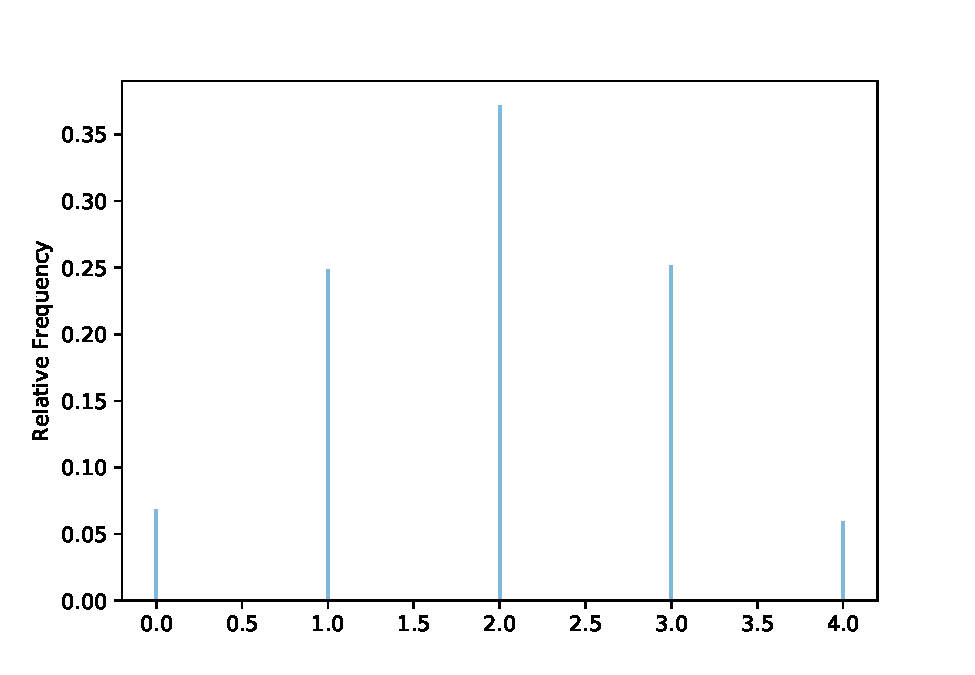
\includegraphics{bookdown-demo_files/figure-latex/unnamed-chunk-5-1.pdf}

\begin{Shaded}
\begin{Highlighting}[]
\BuiltInTok{print}\NormalTok{(x)}
\end{Highlighting}
\end{Shaded}

\begin{verbatim}
## <symbulate.results.RVResults object at 0x000000001D146CC8>
\end{verbatim}

\begin{Shaded}
\begin{Highlighting}[]
\NormalTok{x }\OperatorTok{=}\NormalTok{ RV(Binomial(}\DecValTok{4}\NormalTok{, }\FloatTok{0.5}\NormalTok{)).sim(}\DecValTok{10000}\NormalTok{)}
\NormalTok{plt.figure()}
\NormalTok{x.plot()}
\NormalTok{plt.show()}
\end{Highlighting}
\end{Shaded}

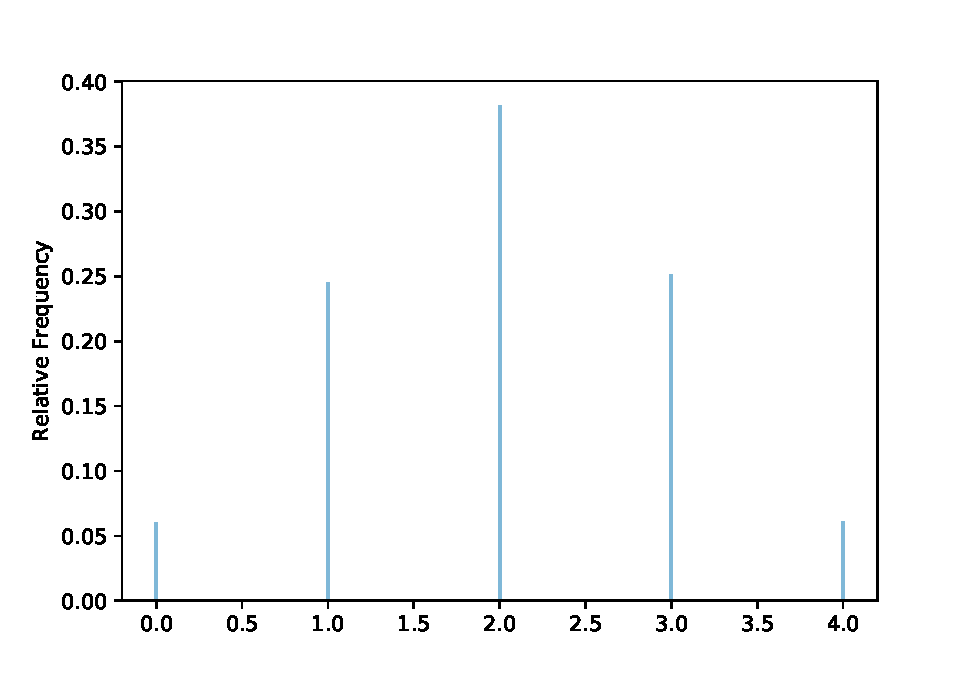
\includegraphics{bookdown-demo_files/figure-latex/unnamed-chunk-6-1.pdf}

\begin{Shaded}
\begin{Highlighting}[]
\BuiltInTok{print}\NormalTok{(x)}
\end{Highlighting}
\end{Shaded}

\begin{verbatim}
## <symbulate.results.RVResults object at 0x000000001C307F48>
\end{verbatim}

would be entered in a Jupyter notebook as

\begin{Shaded}
\begin{Highlighting}[]
\NormalTok{x }\OperatorTok{=}\NormalTok{ RV(Binomial(}\DecValTok{4}\NormalTok{, }\FloatTok{0.5}\NormalTok{)).sim(}\DecValTok{10000}\NormalTok{)}
\NormalTok{x.plot()}
\NormalTok{x}
\end{Highlighting}
\end{Shaded}

\hypertarget{dont-do-what-donny-dont-does}{%
\subsection*{Don't do what Donny Don't does}\label{dont-do-what-donny-dont-does}}
\addcontentsline{toc}{subsection}{Don't do what Donny Don't does}

Some of the examples and exercises in this book are labeled ``Don't do what Donny Don't does''. This is a \href{https://frinkiac.com/video/S05E08/0nvMY69o6o_U7BqeIzQ314al-SQ=.gif}{Simpson's} \href{https://www.youtube.com/watch?v=pbwxlyUunL8}{reference}. In this text, Donny represents a student who makes many of the mistakes commonly made by students studying probability. The idea of these problems is for you to learn from the common mistakes that Donny makes, by identifying why he is wrong and by helping him understand and correct his mistakes. (But be careful: sometimes Donny is right!)

\hypertarget{about-this-book}{%
\subsection*{About this book}\label{about-this-book}}
\addcontentsline{toc}{subsection}{About this book}

This book was written using the \textbf{bookdown} package \citep{R-bookdown}, which was built on top of R Markdown and \textbf{knitr} \citep{xie2015}. Python code was run in RStudio using the \texttt{reticulate} package.

\hypertarget{intro}{%
\chapter{Introduction}\label{intro}}

You can label chapter and section titles using \texttt{\{\#label\}} after them, e.g., we can reference Chapter \ref{intro}. If you do not manually label them, there will be automatic labels anyway, e.g., Chapter \ref{methods}.

Figures and tables with captions will be placed in \texttt{figure} and \texttt{table} environments, respectively.

\begin{Shaded}
\begin{Highlighting}[]
\KeywordTok{par}\NormalTok{(}\DataTypeTok{mar =} \KeywordTok{c}\NormalTok{(}\DecValTok{4}\NormalTok{, }\DecValTok{4}\NormalTok{, }\FloatTok{.1}\NormalTok{, }\FloatTok{.1}\NormalTok{))}
\KeywordTok{plot}\NormalTok{(pressure, }\DataTypeTok{type =} \StringTok{\textquotesingle{}b\textquotesingle{}}\NormalTok{, }\DataTypeTok{pch =} \DecValTok{19}\NormalTok{)}
\end{Highlighting}
\end{Shaded}

\begin{figure}

{\centering 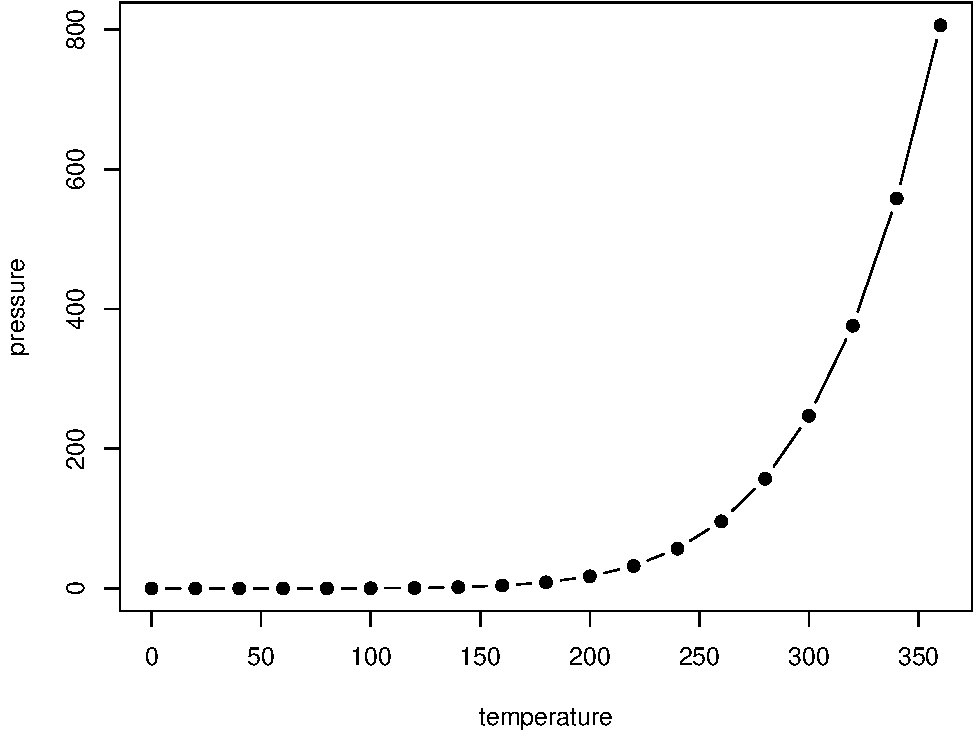
\includegraphics[width=0.8\linewidth]{bookdown-demo_files/figure-latex/nice-fig-1} 

}

\caption{Here is a nice figure!}\label{fig:nice-fig}
\end{figure}

Reference a figure by its code chunk label with the \texttt{fig:} prefix, e.g., see Figure \ref{fig:nice-fig}. Similarly, you can reference tables generated from \texttt{knitr::kable()}, e.g., see Table \ref{tab:nice-tab}.

\begin{Shaded}
\begin{Highlighting}[]
\NormalTok{knitr}\OperatorTok{::}\KeywordTok{kable}\NormalTok{(}
  \KeywordTok{head}\NormalTok{(iris, }\DecValTok{20}\NormalTok{), }\DataTypeTok{caption =} \StringTok{\textquotesingle{}Here is a nice table!\textquotesingle{}}\NormalTok{,}
  \DataTypeTok{booktabs =} \OtherTok{TRUE}
\NormalTok{)}
\end{Highlighting}
\end{Shaded}

\begin{table}

\caption{\label{tab:nice-tab}Here is a nice table!}
\centering
\begin{tabular}[t]{rrrrl}
\toprule
Sepal.Length & Sepal.Width & Petal.Length & Petal.Width & Species\\
\midrule
5.1 & 3.5 & 1.4 & 0.2 & setosa\\
4.9 & 3.0 & 1.4 & 0.2 & setosa\\
4.7 & 3.2 & 1.3 & 0.2 & setosa\\
4.6 & 3.1 & 1.5 & 0.2 & setosa\\
5.0 & 3.6 & 1.4 & 0.2 & setosa\\
\addlinespace
5.4 & 3.9 & 1.7 & 0.4 & setosa\\
4.6 & 3.4 & 1.4 & 0.3 & setosa\\
5.0 & 3.4 & 1.5 & 0.2 & setosa\\
4.4 & 2.9 & 1.4 & 0.2 & setosa\\
4.9 & 3.1 & 1.5 & 0.1 & setosa\\
\addlinespace
5.4 & 3.7 & 1.5 & 0.2 & setosa\\
4.8 & 3.4 & 1.6 & 0.2 & setosa\\
4.8 & 3.0 & 1.4 & 0.1 & setosa\\
4.3 & 3.0 & 1.1 & 0.1 & setosa\\
5.8 & 4.0 & 1.2 & 0.2 & setosa\\
\addlinespace
5.7 & 4.4 & 1.5 & 0.4 & setosa\\
5.4 & 3.9 & 1.3 & 0.4 & setosa\\
5.1 & 3.5 & 1.4 & 0.3 & setosa\\
5.7 & 3.8 & 1.7 & 0.3 & setosa\\
5.1 & 3.8 & 1.5 & 0.3 & setosa\\
\bottomrule
\end{tabular}
\end{table}

You can write citations, too. For example, we are using the \textbf{bookdown} package \citep{R-bookdown} in this sample book, which was built on top of R Markdown and \textbf{knitr} \citep{xie2015}.

\hypertarget{prob-literacy}{%
\chapter{What is Probability?}\label{prob-literacy}}

This chapter provides a non-technical introduction to randomness and probability. Many of the topics introduced in this chapter will be covered in more detail in later chapters.

NO MATH BEYOND TWO WAY TABLES AND BASIC EXPECTED VALUES

Expand chapter 1 with more example of probability/simulation computations with as little math and terminology as possible. (e.g.~Don't define RV or event or sample space.)

Add a few motivating examples with links - 538 election, hurricane, etc

\hypertarget{randomness}{%
\section{Instances of randomness}\label{randomness}}

instances of randomness - examples; include in other sections? (random sampling, random assignment, future/past, etc, physical (coin, die), quantum)

\begin{exercise}
\protect\hypertarget{exr:randomness}{}{\label{exr:randomness} }
Each of the following situations involves a probability. How are the various situations similar, and how are they different? What is one feature that all of the situations have in common? If you were to estimate the probability in question, how might you do it? What are some things to consider? The goal here is not to do any calculations but rather to think about, via these examples, similarities and differences of situations in which probabilities are of interest.
\end{exercise}

\begin{enumerate}
\def\labelenumi{\arabic{enumi}.}
\tightlist
\item
  The probability that a single flip of a fair coin lands on heads.
\item
  The probability that in two flips of a fair coin exactly one flip lands on heads.
\item
  The probability that in 10000 flips of a fair coin exactly 5000 flips land on heads.
\item
  The probability that in 10000 flips of a fair coin ``around'' 5000 flips land on heads.
\item
  The probability you win the next \href{https://www.powerball.com/}{Powerball lottery} if you purchase a single ticket, 6-7-16-23-26, plus the Powerball number, 4. (FYI: There are roughly\footnote{The exact count is 292,201,338. We will see how to compute this number later.} 300 million possible winning number combinations.)
\item
  The probability you win the next Powerball lottery if you purchase a single ticket, 1-2-3-4-5, plus the Powerball number, 6.
\item
  The probability that someone wins the next Powerball lottery. (FYI: especially when the jackpot is large, there are hundreds of millions of tickets sold.)
\item
  The probability that a ``randomly selected'' Cal Poly student is from CA.\\
\item
  The probability that Hurricane Humberto makes landfall in the U.S.
\item
  The probability that the Los Angeles Chargers win the next Superbowl.
\item
  The probability that Donald Trump wins the 2020 U.S. Presidential Election.
\item
  The probability that extraterrestrial life currently exists somewhere in the universe.
\item
  The probability that you ate an apple on April 17, 2009.
\end{enumerate}

\begin{itemize}
\tightlist
\item
  The subject of probability concerns \emph{random} phenomena.
\item
  A phenomenon is \textbf{random} if there are multiple potential outcomes, and there is \textbf{uncertainty} about which outcome will occur. \emph{Uncertainty} is the feature that all the scenarios have in common.
\item
  Uncertainty does not necessarily mean uncertainty about an occurrence in the future. For example, you either ate or apple or not on April 17, 2009, but you're not certain about it. But if you tended to eat a lot of apples ten years ago, then you might give a high probability to the event that you ate one on April 17, 2009.
\item
  Many phenomena involve physical randomness\footnote{We will refer to as ``random'' any scenario that involves a reasonable degree of uncertainty. We're avoiding philosophical questions about what is ``true'' randomness, like the following. Is a coin flip really random? If all factors that affect the trajectory of the coin were known precisely, then wouldn't the outcome be determined? Does true randomness only exist in quantum mechanics?}, like flipping a coin or drawing powerballs at random from a bin.
\item
  Statistical applications often involve the planned use of physical randomness

  \begin{itemize}
  \tightlist
  \item
    \textbf{Random selection} involves selecting a \emph{sample} of individuals at random from a \emph{population} (e.g.~via random digit dialing).
  \item
    \textbf{Random assignment} involves assigning individuals at random to groups (e.g.~in a randomized experiment).
  \end{itemize}
\item
  However, in many other situations randomness just vaguely reflects uncertainty.
\item
  In any case, random does \emph{not} mean haphazard. In a random phenomenon, while
  individual outcomes are uncertain, there is a \emph{regular distribution of
  outcomes over a large number of (hypothetical) repetitions}.

  \begin{itemize}
  \tightlist
  \item
    In two flips of a fair coin we wouldn't necessarily see one head and one tail. But in 10000 flips of a fair coin, we would expect to see close to 5000 heads and 5000 tails.
  \item
    We don't know who will win the next Superbowl, but we can and should certainly consider some teams as more likely to win than others. We could imagine a large number of hypothetical 2019 seasons; how often would we expect the Eagles to win? The Raiders? (Hopefully a lot for the Eagles; probably not much for the Raiders).
  \end{itemize}
\item
  Also, random does \emph{not} necessarily mean equally likely. In a random
  phenomenon, certain outcomes or events might be more or less likely than
  others.

  \begin{itemize}
  \tightlist
  \item
    It's much more likely that a randomly selected Cal Poly student is from CA than not.
  \item
    Not all NFL teams are equally likely to win the next Superbowl.
  \end{itemize}
\end{itemize}

\hypertarget{interpretations}{%
\section{Interpretations of probability}\label{interpretations}}

In the previous section we encountered a variety of scenarios which involved uncertainty, a.k.a. randomness. Just as there are a few ``types'' of randomness, there are a few ways of interpreting probability, namely, \emph{long run relative frequency} and \emph{subjective probability}.

\begin{exercise}
\protect\hypertarget{exr:probability-intepret}{}{\label{exr:probability-intepret} }
Revisit the scenarios in Exercise \ref{exr:randomness}. Now consider how ``probability'' is interpreted in the different scenarios. In each scenario, what does ``probability'' mean? How might you estimate the probability? Start to make guesses for the probabilities; are they ``high'' or ``low''? How high or low? Again, the goal is not to do any calculations but rather to think about, via these examples, similarities and differences of situations in which probabilities are of interest.
\end{exercise}

In particular, compare

\begin{enumerate}
\def\labelenumi{\alph{enumi}.}
\tightlist
\item
  Scenarios 3 and 4
\item
  Scenarios 5 and 6
\item
  Scenarios 6 and 7
\item
  How are scenarios 1 through 8 (collectively) different from scenarios 9 through 13 (collectively)?
\end{enumerate}

\begin{itemize}
\tightlist
\item
  The \textbf{probability} of an event is a number in the interval \([0, 1]\) measuring the event's likelihood or degree of uncertainty.
\item
  A probability can take any values in the continuous scale from 0\% to 100\%\footnote{Probabilities are usually defined as decimals, but are often colloquially referred to as percentages. We're not sticklers; we'll refer to probabilities as decimals and as percentages.}. In particular, a probability requires much more interpretation than ``is the probability greater than, less than, or equal to 50\%?''
\item
  When interpreting probabilities, be careful not to confuse ``the particular'' with ``the general''.

  \begin{itemize}
  \tightlist
  \item
    (``The particular.'') A very specific event, surprising or not, often has low probability.

    \begin{itemize}
    \tightlist
    \item
      Even though in 10000 flips of a fair coin we would expect to see about 5000 heads, the probability that \emph{exactly} 5000 out of 10000 flips are heads is fairly small (about\footnote{We will see how to compute probabilities like this one in upcoming chapters.} 0.008).
    \item
      The probability that the winning powerball number is 6-7-16-23-26-(4) is exactly the same as the probability that the winning powerball number is 1-2-3-4-5-(6). Each of these sequences is just one of the roughly 300 million possible sequences, and each sequences has about a 1 in 300 million chance of being the winning number. However, many people think 6-7-16-23-26-(4) is more likely because 1-2-3-4-5-(6) ``doesn't look random''.
    \item
      The probability that you get a text from your best friend at 7:43pm on Oct 12, 2019 inviting you to dinner after you've just ordered pizza from your favorite pizza place is probably pretty small. None of these items --- getting a text, having a friend invite you to dinner, ordering pizza from your favorite pizza place --- is unusual, but the chances of them all combining in this way at this particular time are fairly small.
    \end{itemize}
  \item
    (``The general.'') However, if there are many like events, their combined probability can be high.

    \begin{itemize}
    \tightlist
    \item
      The probability that \emph{around} 5000 out of 10000 coin flips land on heads is fairly large. For example, if ``around'' is interpreted as between 4900 and 5100 (for a proportion of heads between 0.49 to 0.51) the probability is about 0.956.
    \item
      The probability that the winning powerball number is an ordered sequence, like 1-2-3-4-5-(6), is extremely small\footnote{If a ``sequence'' is defined with the powerball as the last number in the sequence, then the probability is about 21 out of 300 million. Since the powerball must be a number from 1 to 26, there are only 21 tickets out of 300 million possibilities for which the numbers are in an ordered sequence: 1-2-3-4-5-(6), 2-3-4-5-6-(7), \ldots{} 21-22-23-24-25-(26).}. However, the probability that the winning number is not an ordered sequence, like 6-7-16-23-26-(4), is exremely high. When interpreting probabilities, be careful not to confuse an event like ``the winning number is 6-7-16-23-26-(4)'' (the particular, low probability) with an event like ``the winning number is not an ordered sequence'' (the general, high probability).\\
    \item
      The probability that some time in the next month or so a friend invites you for dinner after you've already had dinner on your own is probably fairly high.
    \end{itemize}
  \end{itemize}
\item
  Even if an event has extremely small probability, given enough
  repetitions of the random phenomenon, the probability that the event occurs
  on \emph{at least one} of the repetitions is high.

  \begin{itemize}
  \tightlist
  \item
    The probability that a specific powerball ticket is the winning number is about 1 in 300 million. So if you buy a single ticket, it is \href{https://www.huffpost.com/entry/chances-of-winning-powerball-lottery_b_3288129}{extremely unlikely} that \emph{you} will win.
  \item
    However, if hundreds of millions of powerball tickets are sold, the probability that \emph{someone somewhere} wins is pretty high. For example, if 500 million tickets are sold then there is a roughly 80\% chance that at least one ticket has the winning number (under \href{https://fivethirtyeight.com/features/new-powerball-odds-could-give-america-its-first-billion-dollar-jackpot/}{certain assumptions}).
  \end{itemize}
\end{itemize}

\hypertarget{rel-freq}{%
\subsection{Relative frequency}\label{rel-freq}}

The probability that a single flip of a fair coin lands on heads is 0.5. How do we interpret this 0.5? The notation of ``fairness'' implies that the two outcomes, heads and tails, should be equally likely, so we have a ``50/50 chance''. But how else can we interpret this 50\%? One way is by considering \emph{what would happen if we flipped the coin main times}. Now, if we would flipped the coin twice, we wouldn't expect to necessarily see one head and one tail. And we already mentioned that if we flipped the coin 10000 times, the chances of seeing \emph{exactly} 5000 heads is small. But in many flips, we might expect to see heads on something close to 50\% of flips.

Consider Figure \ref{fig:coin-sim1} below. Each dot represents a set of 10,000 fair coin flips. There are 100 dots displayed, representing 100 different sets of 10,000 coin flips each. For each set of flips, the proportion of the 10,000 flips which landed on head is recorded. For example, if in one set 4973 out of 10,000 flips landed on heads, the proportion of heads is 0.4973. The plot displays 100 such proportions. We see that only 5 of these 100 proportions are less than 0.49 or greater than 0.51. So if between 0.49 and 0.51 is considered ``close to 0.5'', then yes, in 10000 coin flips we would expect the proportion of heads to be close to 0.5. (In 10000 flips, the probability of heads on between 49\% and 51\% of flips is 0.956, so 95 out of 100 provides a rough estimate of this probability.)



\begin{figure}
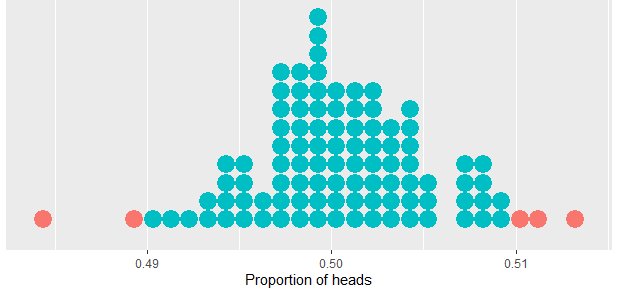
\includegraphics[width=8.65in]{_graphics/coin-sim1} \caption{Proportion of flips which are heads in 100 sets of \textbf{10,000} fair coin flips. Each dot represents a set of \textbf{10,000} fair coin flips.}\label{fig:coin-sim1}
\end{figure}

But what if we want to be stricter about what qualifies as ``close to 0.5''? You might suspect that with even more flips we would expect to observe heads on even closer to 50\% of flips. Indeed, this is the case. Figure \ref{fig:coin-sim2} displays the results of 100 sets of 1,000,000 fair coin flips. The pattern seems similar to Figure \ref{fig:coin-sim1} but pay close attention to the horizontal axis which covers a much shorter range of values than in the previous figure. Now 96 of the 100 proportions are between 0.499 and 0.501. So in 1,000,000 flips we would expect the proportion of heads to be between 0.499 and 0.501, pretty close to 0.5. (In 1,000,000 flips, the probability of heads on between 49.9\% and 50.1\% of flips is 0.955, and 96 out of 100 sets provides a rough estimate of this probability.)



\begin{figure}
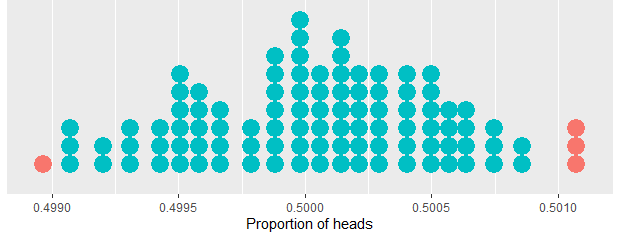
\includegraphics[width=8.65in]{_graphics/coin-sim2} \caption{Proportion of flips which are heads in 100 sets of \textbf{1,000,000} fair coin flips. Each dot represents a set of \textbf{1,000,000} fair coin flips.}\label{fig:coin-sim2}
\end{figure}

In Figure \ref{fig:coin-sim3} each dot represents a set of 100 millions flips. The pattern seems similar to the previous figures, but again pay close attention the horizontal access which covers a smaller range of values. Now 96 of the 100 proportions are between 0.4999 and 0.5001. (In 100 million flips, The probability of heads on between 49.99\% and 50.01\% of flips is 0.977, so 96 out of 100 sets provides a rough estimate of this probability.)



\begin{figure}
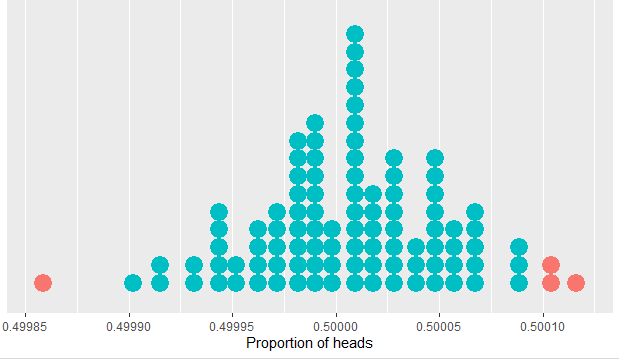
\includegraphics[width=8.6in]{_graphics/coin-sim3} \caption{Proportion of flips which are heads in 100 sets of \textbf{100,000,000} fair coin flips. Each dot represents a set of \textbf{100,000,000} fair coin flips.}\label{fig:coin-sim3}
\end{figure}

The previous figures illustrate that the more flips there are, the more likely it is that we observe a proportion of flips landing on heads close to 0.5. We also see that with more flips we can refine our definition of ``close to 0.5'': increasing the number of flips by a factor of 100 (10,000 to 1,000,000 to 100,000,000) seems to give us an additional decimal place of precision (\(0.5\pm0.01\) to \(0.5\pm 0.001\) to \(0.5\pm 0.0001\).) These observations illustrate the relative frequency interpretation of probability.

\begin{itemize}
\tightlist
\item
  The probability of an event corresponding to the result of a random phenomenon can be interpreted as the proportion of times that the event would occur in a very large number of hypothetical repetitions of the random phenomenon.
\item
  That is, a probability can be interpreted as a \textbf{long run proportion} or \textbf{long run relative frequency}.
\item
  This means that the probability of an event can be approximated by \textbf{simulating} the random phenomenon a large number of times and determining the proportion of simulated repetitions on which the event occurred out of the total number of repetitions of the simulation (this proportion is also called the relative frequency of the event.)

  \begin{itemize}
  \tightlist
  \item
    A \textbf{simulation} involves an artificial recreation of the random phenomenon, usually using a computer.
  \item
    For example, if a basketball player is successful on 90\% of her free throw attempts, we can simulate the player shooting a single free throw attempt by taking 10 cards and labeling 9 as ``success'' and 1 as ``miss'' then shuffling well and dealing one card.
  \end{itemize}
\item
  The \textbf{long run relative frequency} interpretation of probability can be applied when a situation can be repeated numerous times, at least conceptually, and the outcome can be observed each time.
\item
  The relative frequency of a particular event will settle down to a single constant value after many repetitions, and that long run value is the probability of that event.

  \begin{itemize}
  \tightlist
  \item
    However, what constitutes the random phenomenon or how the simulation is conducted depends on certain assumptions. Changing those assumptions can affect probabilities of interest.

    \begin{itemize}
    \tightlist
    \item
      For example, if you're interested in the probability that a die lands on 1, you need to know if it's a four-sided die or a six-sided die, and if the die is consider ``fair''.
    \item
      As a more complicated example, simulating the outcome of the next Superbowl involves many assumptions
    \end{itemize}
  \end{itemize}
\end{itemize}

\hypertarget{subjective-probability}{%
\subsection{Subjective probability}\label{subjective-probability}}

The relative frequency interpretation is natural in scenarios 1 through 8 of Exercise \ref{exr:randomness}. We can consider as repeateable situations like flipping a coin, drawing powerballs from a bin, or selecting a student at random.

On the other hand, it is difficult to conceptualize scenarios 8 through 13 of Exercise \ref{exr:randomness} as relative frequencies. Superbowl 2020 will only be played once, the 2020 U.S. Presidential Election will only be conducted once (we hope), and there was only one April 17, 2009 on which you either did or did not eat an apple. But while these situations are not naturally repeatable they still involve randomness (uncertainty) and it is still reasonable to assign probabilities. At this point in time, the Chargers are less likely than the Patriots (ugh) to win Superbowl 2020, Donald Trump is more likely than Dwayne Johnson to win the U.S. 2020 Presidential Election, and if you've always been an ``apple-a-day'' person, there's a good chance you ate one on April 17, 2009. So it still makes sense to talk about probability in uncertain, but not necessarily repeated situations.

However, the \emph{meaning} of probability does seem different in scenarios 9 through 13 compared to 1 through 8. Consider Superbowl 2020. As of Sept 16,

\begin{itemize}
\tightlist
\item
  According to \href{https://projects.fivethirtyeight.com/2019-nfl-predictions/}{fivethirtyeight.com}, the Patriots have a 19\% chance of winning the Superbowl, the highest of any team, while the Chargers have a 4\% chance.
\item
  According to \href{https://www.footballoutsiders.com/stats/playoffodds}{footballoutsider.com}, the Patriots have a 26\% chance of winning the Superbowl, the highest of any team, while the Chargers have a 6\% chance.
\item
  According to \href{http://www.playoffstatus.com/nfl/nflpostseasonprob.html}{playoffstatus.com} the Patriots have a 7\% chance of winning the Superbowl, behind the Chiefs and Packers at 9\% each, while the Chargers have a 3\% chance.
\end{itemize}

All three websites, as well as many others, ascribe different probabilities to the Patriots or Chargers winning. Which website, if any, is correct? In the coin flipping example, we could perform a simulation to see that the long run relative frequency is 0.5. However, simulating Superbowl 2020 involves first simulating the 2019 season to determine the playoff matchups, then simulating the playoffs to see which teams make the Superbowl, then simulating the Superbowl matchup itself. And simulating the 2019 involves simulating all the weekly matchups and potential injuries and their effects. Even just simulating a single game involves many assumptions; differences in opinions with regards to these assumptions can lead to different probabilities. For example, according to fivethirtyeight, the Chiefs have a 69\% chance of beating the Ravens on Sept 22, but according to pickingpros.com it's only 52\%. Unlike in the coin flipping problem, there is no single set of rules for running the simulation, and there is no single relative frequency that determines the probability. Therefore, in a situation like forecasting the Superbowl we consider \emph{subjective probability}.

\begin{itemize}
\tightlist
\item
  There are many situations where the outcome is uncertain, but it does mnot make sense to consider the situation as repeatable. In such situations, a \textbf{subjective (a.k.a. personal) probability} describes the degree of likelihood a given individual ascribes to a certain event.
\item
  As the name suggests, different individuals might have different subjective (personal) probabilities for the same event.

  \begin{itemize}
  \tightlist
  \item
    In contrast to the long run relative frequency situation, in which the probability is agreed to be defined as the long run relative frequency.
  \end{itemize}
\item
  The \href{https://fivethirtyeight.com/methodology/how-our-nfl-predictions-work/}{fivethirtyeight NFL predictions} are the output of a probabilistic forecast.

  \begin{itemize}
  \tightlist
  \item
    \textbf{Probabilistic forecasts} combine observed data and statistical models to make predictions.
  \item
    Rather than providing a single prediction (such as ``the Patriots will win Superbowl 2020''), probabilistic forecasts provide a range of scenarios and their relative likelihoods.
  \item
    Be sure to make a distinction between \emph{assumption} and \emph{observation}.
  \end{itemize}
\end{itemize}

\hypertarget{proportional-reasoning-and-tables-of-counts}{%
\section{Proportional reasoning and tables of counts}\label{proportional-reasoning-and-tables-of-counts}}

\begin{itemize}
\tightlist
\item
  In general, knowing probabilities of individual events alone is not enough to determine probabilities of combinations of them.
\item
  \textbf{Two-way tables} (a.k.a. contingency tables) of counts are a useful tool for probability problems dealing with two events.
\item
  For the purposes of constructing the table and computing related probabilities, any value can be used for the hypothetical total count (as long as you don't round numbers in between).
\end{itemize}

Suppose we are interested in the relationship between income and college graduation rates at Cal Poly. Consider the sample space \(S = \{\text{all current Cal Poly students}\}\).
Suppose that the probability\footnote{These number are estimates based on data from \url{https://projects.propublica.org/colleges/schools/california-polytechnic-state-university-san-luis-obispo}} that a (randomly selected) Cal Poly student graduates within six years is 0.75, and that the probability that a (randomly selected) Cal Poly student has a Pell grant (for low income students) is 0.2.

\begin{enumerate}
\def\labelenumi{\arabic{enumi}.}
\tightlist
\item
  Do we have enough information to find the probability that a Cal Poly student both has a Pell Grant and graduates within six years?
\item
  Without knowing any other information, what is the \emph{largest} value the probability in (a) could possibly be? Under what conditions is this value attained? Set up a two-way table corresponding to this scenario.
\item
  Without knowing any other information, what is the \emph{smallest} value the probability in (a) could possibly be? Under what conditions is this value attained? Set up a two-way table corresponding to this scenario.
\item
  Suppose that the probability that a Cal Poly student both has a Pell Grant and graduates within six years is 0.11. Construct the corresponding two-way table.
\item
  Find the probability that a Cal Poly student does not have a Pell Grant and graduates within six years.
\item
  Donny says ``75\% of CP students graduate within six years while 20\% of CP students have a Pell Grant. So 95\% of Cal Poly students graduate within six years or have a Pell Grant.'' Do you agree?
\item
  What would need to be true in order for the Donny's statement in the previous part to be true?
\end{enumerate}

\hypertarget{consistency}{%
\section{Working with probabilities}\label{consistency}}

In the previous section we saw two different interpretations of probability: relative frequency and subjective. Fortunately, the mathematics of probability work the same way regardless of the interpretation. Also, even with subjective probabilities it is helpful to consider what might happen in a simulation.

\hypertarget{consistency-requirements}{%
\subsection{Consistency requirements}\label{consistency-requirements}}

With either the relative frequency or personal probability interpretation there are some basic logical consistency requirements\footnote{In Section \ref{probspace}, we will formalize these requirements in the axioms of probability.} which probabilities need to satisfy.

\begin{example}
\protect\hypertarget{exm:worldseries}{}{\label{exm:worldseries} }
As of Sept 18, the website \href{https://projects.fivethirtyeight.com/2019mlb-predictions/}{fivethirtyeight.com} listed the following probabilities for who will
win the 2019 World Series.
\end{example}

\begin{longtable}[]{@{}lr@{}}
\toprule
\endhead
Houston Astros & 25\%\tabularnewline
Los Angeles Dodgers & 21\%\tabularnewline
ew York Yankees & 20\%\tabularnewline
tlanta Braves & 8\%\tabularnewline
\bottomrule
\end{longtable}

\begin{enumerate}
\def\labelenumi{\arabic{enumi}.}
\tightlist
\item
  Is the relative frequency or subjective probability interpretation more appropriate here?
\item
  According to the site, what must be the probability that the Houston Astros do \emph{not} win?
\item
  According to this site, what must be the probability that one of the above four teams is the World Series champion?
\item
  According to this site, what must be the probability that a team other than the above four teams is the World Series champion?
\end{enumerate}

\begin{solution}
\iffalse{} {Solution. } \fi{}
to Example \ref{exm:worldseries}
\end{solution}

\begin{enumerate}
\def\labelenumi{\arabic{enumi}.}
\tightlist
\item
  It is more appropriate to think of the probabilities themselves in application as subjective. Different websites or models could reasonably assign other probabilities to the teams. However, we can still imagine the probabilities as relative frequencies, if it helps our intuition. If we think of this as a simulation, each repetition results in a World Series champion and in the long run the Astros would be the champion in 25\% of repetitions.
\item
  Either the Astros win or they don't; if there's a 25\% chance that the Astros win, there must be a 75\% chance that they do not win. If we think of this as a simulation, each repetition results in either the Astros winning or not, so if they win in 25\% of repetitions, they must not win in the other 75\% to account for 100\% of the repetitions.
\item
  There is only one World Series champion, so if say the Astros win then no other team can win. Thinking again of a simulation, the repetitions in which the Astros win are distinct from those in which the Dodgers win. So if the Astros win in 25\% of repetitions and the Dodgers wins in 21\% repetitions, then on a total of 46\% of repetitions either the Astros or Dodgers win. Adding the four probabilities, we see that the probability that one of the four teams above wins must be 74\%.
\item
  Either one of the four teams above wins, or some other team wins. If there is a 74\% chance that the winner is one of the four teams above, then there must be a 26\% chance that the winner is not one of these four teams.
\end{enumerate}

\hypertarget{odds}{%
\subsection{Odds}\label{odds}}

The words ``probability'', ``chance'', ``likelihood'', and ``odds'' are colloquially treated as synonyms. However, in the mathematical language of probability, \emph{odds} provide a different way of reporting a probability. Rather than reporting probability on a 0\% to 100\% scale, odds report probabilities in terms of ratios.

\begin{example}
\protect\hypertarget{exm:worldseries-odds}{}{\label{exm:worldseries-odds} }
In Example \ref{exm:worldseries} the odds that the Astros win the World Series are 3 to 1 against.
\end{example}

\begin{enumerate}
\def\labelenumi{\arabic{enumi}.}
\tightlist
\item
  What do you think that ``3 to 1 against'' means?
\item
  What are the odds of the Astros \emph{not} winning?
\item
  What are the odds of the Yankees winning?
\item
  What are the odds of the Braves winning?
\end{enumerate}

\begin{solution}
\iffalse{} {Solution. } \fi{}
to Example \ref{exm:worldseries-odds}
\end{solution}

\begin{enumerate}
\def\labelenumi{\arabic{enumi}.}
\tightlist
\item
  The probability that the Astros win is 0.25, so the probability that they do not win is 0.75. These numbers are in a 3 to 1 ratio: the probability of not winning (0.75) is 3 times greater than the probability of winning (0.25). So the odds \emph{against} the Astros winning the World Series are 3 to 1; ``against'' because the Astros are less likely to win than to not win.
\item
  The probabilities are still in the 3 to 1 ratio, but we can say that the odds are 3 to 1 \emph{in favor} of the Astros \emph{not} winning.
\item
  The probability that the Yankees win is 0.2 and that they don't win is 0.8, and \(0.8/0.2 = 4\)). So the odds are 4 to 1 against the Yankees winning (``against'' because the Yankees are less likely to win than to not win).
\item
  The probability that the Braves win is 0.08 and that they don't win is 0.92, and \(0.92/0.08 = 11.5\)). So the odds are 11.5 to 1, or 23 to 2, against the Braves winning (``against'' because the Braves are less likely to win than to not win).
\end{enumerate}

\begin{itemize}
\tightlist
\item
  The \textbf{odds} of an event is a ratio involving the probability that the
  event occurs and the probability that the event does not occur
  \[
  \begin{aligned}
  \text{odds in favor} & = \frac{\text{probability that the event occurs}}{\text{probability that the event does not occur}} \\
  & \\
  \text{odds against} & = \frac{\text{probability that the event does not occur}}{\text{probability that the event  occurs}}\end{aligned}
  \]
\item
  In many situations (e.g., gambling) odds are implicitly reported as odds against.
\item
  Odds are usually expressed as whole numbers, e.g., 11 to 1, 7 to 2.
\end{itemize}

Ron and Leslie make the following bet. If Boston wins, Leslie will pay
Ron \$200; if not, Ron will pay Leslie \$100. If both consider this to
be a fair bet, what have they agreed that the probability that Boston
wins is?

The odds of a fair bet on whether or not an event will occur imply a
probability for the event
\[\text{probability that event occurs} = \frac{\text{odds in favor of the event}}{1+\text{odds in favor of the event}}\]

\hypertarget{dutch-book}{%
\subsection{Dutch book}\label{dutch-book}}

Dutch book\footnote{``Book'' in the sense of a bookie taking bets}

Odds give us one way to see why even subjective probabilities most follow basic logical consistency requirements.

\begin{example}
\protect\hypertarget{exm:dutch}{}{\label{exm:dutch} }
Donny Dont is pretty sure that the Astros are going to win the World Series. He thinks their only real competition is the Braves. The following are Donny's subjective probabilities.

\begin{longtable}[]{@{}lr@{}}
\toprule
\endhead
Houston Astros & 60\%\tabularnewline
Atlanta Braves & 20\%\tabularnewline
Other & 10\%\tabularnewline
\bottomrule
\end{longtable}
\end{example}

\hypertarget{sim}{%
\section{Approximating probabilities - a brief introduction to simulation}\label{sim}}

Here's a seemingly simple problem. Flip a fair coin four times and record the results in order. For the recorded sequence, compute \emph{the proportion of the flips which immediately follow a H that result in H}. What value do you expect for this proportion? (If there are no flips which immediately follow a H, i.e.~the outcome is either TTTT or TTTH, discard the sequence and try again with four more flips.)

For example, the sequence HHTT means the the first and second flips are heads and the third and fourth flips are tails. For this sequence there are two flips which immediately followed heads, the second and the third, of which one (the second) was heads. So the proportion in question for this sequence is 1/2.

So what value do you expect for this proportion? We think it's safe to say that most people would answer 1/2. Afterall, it shouldn't matter if a flip follows heads or not, right? We would expect half of the flips to land on heads regardless of whether the flip follows H, right? We'll see there are some subtleties lurking behind these questions.

To get an idea of what we would expect for this proportion, we could conduct a simulation: flip a coin 4 times and see what happens. Here are the results of a few repetitions; each repetition consists of an ordered sequence of 4 coin flips for which the proportion in question is measured. (\textbf{Flips which immediately follow H are in bold.})

\begin{longtable}[]{@{}rrllr@{}}
\caption{\label{tab:mscoin-intro} Simulated outcomes for 6 sets of four flips of a fair coin.}\tabularnewline
\toprule
\begin{minipage}[b]{0.12\columnwidth}\raggedleft
Repetition \textbar{}\strut
\end{minipage} & \begin{minipage}[b]{0.10\columnwidth}\raggedleft
Outcome \textbar{} Fl\strut
\end{minipage} & \begin{minipage}[b]{0.20\columnwidth}\raggedright
Flips that follow H \textbar{}\strut
\end{minipage} & \begin{minipage}[b]{0.16\columnwidth}\raggedright
H that follow H \textbar{} Pro\strut
\end{minipage} & \begin{minipage}[b]{0.28\columnwidth}\raggedleft
Proportion of H following H \textbar{}\strut
\end{minipage}\tabularnewline
\midrule
\endfirsthead
\toprule
\begin{minipage}[b]{0.12\columnwidth}\raggedleft
Repetition \textbar{}\strut
\end{minipage} & \begin{minipage}[b]{0.10\columnwidth}\raggedleft
Outcome \textbar{} Fl\strut
\end{minipage} & \begin{minipage}[b]{0.20\columnwidth}\raggedright
Flips that follow H \textbar{}\strut
\end{minipage} & \begin{minipage}[b]{0.16\columnwidth}\raggedright
H that follow H \textbar{} Pro\strut
\end{minipage} & \begin{minipage}[b]{0.28\columnwidth}\raggedleft
Proportion of H following H \textbar{}\strut
\end{minipage}\tabularnewline
\midrule
\endhead
\begin{minipage}[t]{0.12\columnwidth}\raggedleft
1 \textbar{}\strut
\end{minipage} & \begin{minipage}[t]{0.10\columnwidth}\raggedleft
H\textbf{HT}T \textbar{}\strut
\end{minipage} & \begin{minipage}[t]{0.20\columnwidth}\raggedright
2 \textbar{}\strut
\end{minipage} & \begin{minipage}[t]{0.16\columnwidth}\raggedright
1 \textbar{}\strut
\end{minipage} & \begin{minipage}[t]{0.28\columnwidth}\raggedleft
0.5 \textbar{}\strut
\end{minipage}\tabularnewline
\begin{minipage}[t]{0.12\columnwidth}\raggedleft
2 \textbar{}\strut
\end{minipage} & \begin{minipage}[t]{0.10\columnwidth}\raggedleft
H\textbf{T}TH \textbar{}\strut
\end{minipage} & \begin{minipage}[t]{0.20\columnwidth}\raggedright
1 \textbar{}\strut
\end{minipage} & \begin{minipage}[t]{0.16\columnwidth}\raggedright
0 \textbar{}\strut
\end{minipage} & \begin{minipage}[t]{0.28\columnwidth}\raggedleft
0 \textbar{}\strut
\end{minipage}\tabularnewline
\begin{minipage}[t]{0.12\columnwidth}\raggedleft
3 \textbar{}\strut
\end{minipage} & \begin{minipage}[t]{0.10\columnwidth}\raggedleft
TTTH \textbar{}\strut
\end{minipage} & \begin{minipage}[t]{0.20\columnwidth}\raggedright
0 \textbar{}\strut
\end{minipage} & \begin{minipage}[t]{0.16\columnwidth}\raggedright
NA \textbar{}\strut
\end{minipage} & \begin{minipage}[t]{0.28\columnwidth}\raggedleft
try again \textbar{}\strut
\end{minipage}\tabularnewline
\begin{minipage}[t]{0.12\columnwidth}\raggedleft
4 \textbar{}\strut
\end{minipage} & \begin{minipage}[t]{0.10\columnwidth}\raggedleft
TH\textbf{HH} \textbar{}\strut
\end{minipage} & \begin{minipage}[t]{0.20\columnwidth}\raggedright
2 \textbar{}\strut
\end{minipage} & \begin{minipage}[t]{0.16\columnwidth}\raggedright
2 \textbar{}\strut
\end{minipage} & \begin{minipage}[t]{0.28\columnwidth}\raggedleft
1 \textbar{}\strut
\end{minipage}\tabularnewline
\begin{minipage}[t]{0.12\columnwidth}\raggedleft
5 \textbar{}\strut
\end{minipage} & \begin{minipage}[t]{0.10\columnwidth}\raggedleft
H\textbf{HT}T \textbar{}\strut
\end{minipage} & \begin{minipage}[t]{0.20\columnwidth}\raggedright
2 \textbar{}\strut
\end{minipage} & \begin{minipage}[t]{0.16\columnwidth}\raggedright
1 \textbar{}\strut
\end{minipage} & \begin{minipage}[t]{0.28\columnwidth}\raggedleft
0.5 \textbar{}\strut
\end{minipage}\tabularnewline
\begin{minipage}[t]{0.12\columnwidth}\raggedleft
6 \textbar{}\strut
\end{minipage} & \begin{minipage}[t]{0.10\columnwidth}\raggedleft
H\textbf{HHT} \textbar{}\strut
\end{minipage} & \begin{minipage}[t]{0.20\columnwidth}\raggedright
3 \textbar{}\strut
\end{minipage} & \begin{minipage}[t]{0.16\columnwidth}\raggedright
2 \textbar{}\strut
\end{minipage} & \begin{minipage}[t]{0.28\columnwidth}\raggedleft
0.667 \textbar{}\strut
\end{minipage}\tabularnewline
\bottomrule
\end{longtable}

We can keep repeating the above process to investigate what happens in the long run. Rather than actually flipping coins, we use a computer to run a simulation. The table and plot below summarize the results of 1,000,000 repetitions of the simulation\footnote{Section XXX covers how to program the simulation and analyze the results.}. While you can't see the individual ``dots'' in the plot, each dot would represent a sequence of 4 coin flips (with at least one flip following a H) and the value plotted being plotted is the proportion of H following H for that sequence. The results could be summarized in a table like Table \ref{tab:mscoin-intro}, albeit with 1,000,000 rows (after discarding rows with no flips immediately following H.)



\begin{figure}
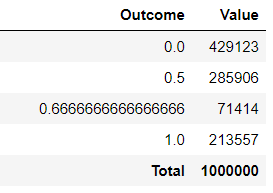
\includegraphics[width=0.5\linewidth]{_graphics/mscoin-intro-table} 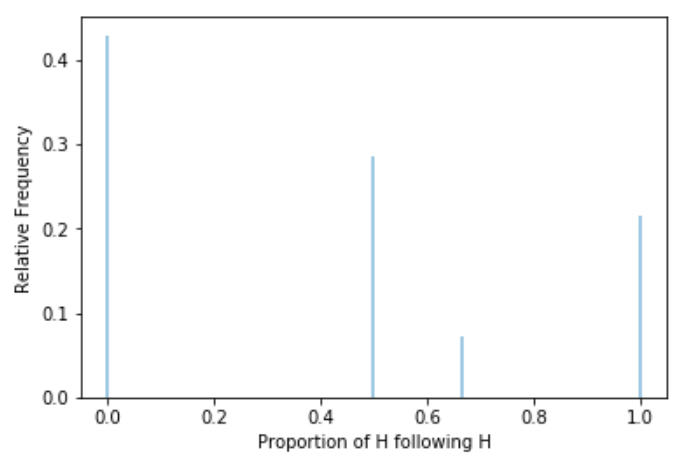
\includegraphics[width=0.5\linewidth]{_graphics/mscoin-intro-plot} \caption{Proportion of flips immediately following Heads that result in Heads for 1,000,000 sets of 4 coin flips. (Each set has at least one flip immediately following H.) For example, the proportion in 429,123 of sets}\label{fig:ms-coin-intro-plot}
\end{figure}

We asked the question: \emph{what would you expect} for the proportion of the flips which immediately follow a H that result in H? That depends on how we define what's ``expected''. If we are interested in the value that is most likely to occur when we flip a coin four times, then the answer is 0: we see that in the long run a little over 40\% of the sets resulted in a proportion of 0, while only about 30\% of sets resulted in a value of 1/2. We see that the plot is not centered at 1/2; a higher percentage of repetitions resulted in a proportion below 1/2 than above 1/2. We think that most people would find this surprising.

Another way to interpret ``expected'' is as ``average''. Just as probability can be interpreted as long run relative frequency, there is a concept called \emph{expected value} which can be interpreted as the \emph{long run average value}. After 1,000,000 repetitions, each involving a set of four fair coin flips, we have 1,000,000 simulated values of the proportion of H following H, as recorded in the rightmost column of Table \ref{tab:mscoin-intro}. We could then average these values: add up the values in the column and divide by 1,000,000. It turns out that average value is 0.405, which is not 1/2. Again, we think most people find this surprising.

A quick note: the term ``expected value'' is somewhat of a misnomer. We are \emph{not} saying that if we flip a coin four times we would expect the proportion of H following H for that set of flips to be 0.405. In fact, the simulation shows that on any single set of four fair coin flips, the only possible values for the proportion of H following H are 0, 1/2, 2/3, and 1. So in a set of four coin flips it's not possible to see a proportion of 0.405. Rather, 0.405 is the \emph{average value of the proportion of H following H that we would expect to see in the long run over many sets of four fair coin flips}. We will return to this idea later.

We will return to this example several times throughout the book to investigate these results more closely. For now, just observe that

\begin{itemize}
\tightlist
\item
  The study of probability can involve some subtleties and our intuition isn't always right.
\item
  Simulation is an effective way of investigating probability problems, and can reveal interesting and suprising patterns.
\end{itemize}

In MS coin - add statement about probability of H after H versus proportion of H after H

\hypertarget{sliding-scale-of-probability-or-probability-of-what}{%
\section{Sliding scale of probability, or Probability of what?}\label{sliding-scale-of-probability-or-probability-of-what}}

\href{https://mathwithbaddrawings.com/2015/09/23/what-does-probability-mean-in-your-profession/}{Here's a funny series of cartoons}

What does 1/million mean?

At least one, etc.

xkcd/538 benchmarks, put in benchmarks (one in a million, a billion, etc)

probability of coincidences

\hypertarget{common-misinterpretation-and-fallacies-e.g.-outbreak-of-asian-disease-utts-book}{%
\section{Common misinterpretation and fallacies (e.g.~outbreak of Asian disease, Utts book)}\label{common-misinterpretation-and-fallacies-e.g.-outbreak-of-asian-disease-utts-book}}

Sally Clark?

Allais paradox?

A famous study\footnote{Source: \url{https://www.ncbi.nlm.nih.gov/pubmed/7455683}} by Kahneman and Tversky presented a group of people
with the following scenario.\\
~\\
"Imagine that the U.S. is preparing for the outbreak of an unusual Asian
disease, which is expected to kill 600 people. Two alternative programs
to combat the disease have been proposed. Assume that the exact
scientific estimate of the consequences of the programs are as follows:

If Program A is adopted, 200 people will be saved.

If Program B is adopted, there is 1/3 probability that 600 people will
be saved, and 2/3 probability that no people will be saved.

Which of the two programs would you favor?"\\

Which of these two options, A or B, would you choose? Of the 152
participants, a large majority (72\%) favored one of the options; which
one do you think it was?

A second group was presented with the same set up, but the following
options instead of A/B.\\

If Program C is adopted 400 people will die.

If Program D is adopted there is 1/3 probability that nobody will die,
and 2/3 probability that 600 people will die.\\

Which of these two options, C or D, would you choose? Of the 155
participants, a large majority (78\%) favored one of the options; which
one do you think it was?

Compute the expected number of people who die and who are saved with
Program D.

Compute the expected number of people who die and who are saved with
Program B.

Compare options A and C. Are these the same? How about B and D? Do the
risk preferences depend on the wording of how the information is
presented?

Many studies have shown that human intuition does not generally deal
well with issues of uncertainty.

So it's worthwhile to take a careful study

\begin{example}[Monty Hall problem]
\protect\hypertarget{exm:monty-hall}{}{\label{exm:monty-hall} \iffalse (Monty Hall problem) \fi{} }MOnty Hall in CHpater 1???
\end{example}

\hypertarget{why-study-coins-dice-cards-and-spinners}{%
\section{Why study coins, dice, cards, and spinners?}\label{why-study-coins-dice-cards-and-spinners}}

Many probability problems involve ``toy'' situations like flipping coins, rolling dice, shuffling cards, or spinning spinners. These situations might seem unexciting, or at least not very practically meaningful. However, coins and spinners and the like provide familiar, concrete situations which facilitate understanding of probability concepts. Furthermore, simple situations often provide insight into real and complex problems. The following is just one illustration.

Many basketball players and fans alike believe in the ``hot hand''
phenomenon: the idea that making several shots in a row increases a
player's chances of making the next shot. However, the consensus
conclusion of thirty years of studies on the hot hand, beginning with
the seminal study \citet{GVT}, had been that there is
no statistical evidence that the hot hand in basketball is real. As a
result, many statisticians regularly caution against the ``hot hand
fallacy'': the belief that the hot hand exists when, in reality, the
degree of streaky behavior typically observed in sequential data is
consistent with what would be expected simply by chance in independent
trials.

The idea behind studies like \citet{GVT} is essentially the
following. Consider a player who attempts 100 shots and makes 50\%. If
there is no hot hand, then we might expect the player to make 50\% of
shots both on attempts that follow hit streaks --- usually considered
three (or more) made attempts in a row --- and on other attempts.
Therefore, a success rate of 50\% on both sets of attempts provides no
evidence of the hot hand.

However, recent research of \citet{MStruth}, \citet{MSthree}, \citet{MScold} concludes that previous studies on the hot hand in basketball,
starting with \citet{GVT}, have been subject to a bias. After
correcting for the bias, the authors find strong evidence in favor of
the hot hand effect in basketball shooting, suggesting the hot hand
fallacy is not a fallacy after all. One interesting aspect of these
studies is that Miller and Sanjurjo's methods are simulation-based.

\citet{MStruth} introduced the coin flipping problem in Section \ref{sim} to illustrate the idea behind their research and the
bias in previous studies. Consider again a player who attempts 100 shots
and makes 50\%. Even if there is no hot hand, Miller and Sanjurjo show that we would actually expect the player to have a shooting percentage of \emph{strictly less than} 50\% on the attempts which followed streaks, and strictly greater than 50\% on the other attempts. The reason is the same as for the coin flipping problem in Section \ref{sim}: in a fixed number of trials, the proportion of H on trials following H is expected to be less than the true probability of H, even though the trials are independent. Therefore, for the example player a success rate of 50\% on both sets of attempts actually provides directional evidence in favor of the hot hand. Properly acccounting for this bias leads to substantially different statistical analyses (i.e., p-values) and conclusions.

\hypertarget{probmath}{%
\chapter{The Language of Probability}\label{probmath}}

CHANGE EVAL TO TRUE AFTER FIGURE PYTHON ERRORS OUT

This chapter introduces the fundamental terminology, objects, and mathematics of random phenomena.

\hypertarget{samplespace}{%
\section{Sample space of outcomes}\label{samplespace}}

A phenomenon is \textbf{random} if there are multiple potential
\emph{outcomes}, and there is \emph{uncertainty} about which outcome will occur. Because there is wide variety in types of random phenomna, an outcome can be virtually anything:

\begin{itemize}
\tightlist
\item
  a sequence of coin flips
\item
  a shuffle of a deck of cards
\item
  the weather tomorrow in your city
\item
  the path of a hurricane
\item
  a sample of registered voters
\item
  player locations over time in an NBA game (as recorded by the \href{https://www.stats.com/sportvu-basketball/}{SportsVU system})
\end{itemize}

And on and on. In particular, an outcome does \emph{not} have to be a number.

The first step in defining a model for a random phenomenon is to describe the possible outcomes.

\begin{definition}
\protect\hypertarget{def:sample-space}{}{\label{def:sample-space} }
The \textbf{sample space}, denoted \(\Omega\) (the uppercase Greek letter ``omega''), is the set of all possible
outcomes of a random phenomenon. An \textbf{outcome}, denoted \(\omega\) (the lowercase Greek letter ``omega''), is an element of the sample space: \(\omega\in\Omega\).
\end{definition}

Mathematically, the sample space \(\Omega\) is a \emph{set} containing all possible outcomes, while an indvidual outcome \(\omega\) is a \emph{point} or \emph{element} in \(\Omega\). The symbol \(\omega\) denotes a generic outcome, much like the symbol \(u\) in \(\sqrt{u}\) denotes a generic input to the square root function.

For example, the simplest random phenomena have just two distinct outcomes, in which case the sample space is just a set with two elements, e.g.~\(\Omega=\{\text{no}, \text{yes}\}\), \(\Omega=\{\text{off}, \text{on}\}\), \(\Omega=\{0, 1\}\), \(\Omega=\{-1, 1\}\). For example, the sample space for a single coin flip could be \(\Omega = \{H, T\}\). If the coin lands on heads, we observe the outcome \(\omega = H\); if tails we observe \(\omega=T\).

A random phenomenon is modeled by a \emph{single} sample space, upon which all objects are defined. These objects, which we will encounter later, include events, random variables, stochastic processes.

Whenever possible, a sample space outcome should be defined to provide the maximum amount of information about the outcome of random phenomenon. While a random phenomenon always has a corresponding sample space, we will see that in many situations the sample space of outcomes is at best only vaguely specified and can not be feasibly enumerated.

\begin{example}
\protect\hypertarget{exm:dice-outcome}{}{\label{exm:dice-outcome} }
Roll a four-sided die\footnote{Why four-sided? Simply to make the number of possibilities a little more manageable (e.g., for in-class simulation activities). Rolling a four-sided die twice yields 16 possible pairs, while rolling a six-sided die yields 36 possible pairs.} twice, and record the result of each roll in sequence as an ordered pair. For example, the outcome \((3, 1)\) represents a 3 on the first roll and a 1 on the second; this is not the same outcome as \((1, 3)\).
\end{example}

\begin{enumerate}
\def\labelenumi{\arabic{enumi}.}
\tightlist
\item
  Identify the sample space.
\item
  We might be interested in the sum of the two dice. Explain why it is still advantageous to define the sample space as in the previous part, rather than as \(\Omega=\{2, \ldots, 8\}\).
\end{enumerate}

\begin{solution}
\iffalse{} {Solution. } \fi{}to Example \ref{exm:dice-event}
\end{solution}

\begin{enumerate}
\def\labelenumi{\arabic{enumi}.}
\tightlist
\item
  The sample space consists of 16 possible ordered pairs of rolls
\end{enumerate}

\begin{align*}
\Omega & = \{(1, 1), (1, 2), (1, 3), (1, 4),\\
& \qquad (2, 1), (2, 2), (2, 3), (2, 4),\\
& \qquad (3, 1), (3, 2), (3, 3), (3, 4),\\
& \qquad (4, 1), (4, 2), (4, 3), (4, 4)\}
\end{align*}

It is more helpful to represent the above set in a table like the following

\begin{enumerate}
\def\labelenumi{\arabic{enumi}.}
\tightlist
\item
  Yes, we might be interested in the sum of the two dice. But we might also be interested in other things, like the larger of the two rolls, or if at least one 3 was rolled, or the first number rolled. Knowing just the sum of the dice does not provide as much information about the outcome of the random phenomenon as the sequence of individual rolls does.
\end{enumerate}

\textbf{Note:} In the previous example, there was a single sample space whose outcomes represented the result of the pair of rolls. In particular, there was not a separate sample space for each of the individual rolls. Now, we could have written the sample space as the Cartesian product \(\Omega = \{1, 2, 3, 4\} \times\{1, 2, 3, 4\}\), where the first, respectively second, set the in the product represents the result of the first, respectively second, roll. But this Cartesian product represents a single set of ordered pairs, and it is that single set which is the sample space corresponding to outcomes of the pair of rolls.

\begin{example}
\protect\hypertarget{exm:coin-outcome}{}{\label{exm:coin-outcome} }
Consider the outcome of a sequence of 4 flips of a coin.
\end{example}

\begin{enumerate}
\def\labelenumi{\arabic{enumi}.}
\tightlist
\item
  Identify an appropriate sample space.
\item
  We might be interested in the number of heads flipped. Explain why it is still advantageous to define the sample space as in the previous part, rather than as \(\Omega=\{0, 1, 2, 3, 4\}\).
\end{enumerate}

\begin{solution}
\iffalse{} {Solution. } \fi{}to Example \ref{exm:coin-outcome}
\end{solution}

\begin{enumerate}
\def\labelenumi{\arabic{enumi}.}
\tightlist
\item
  An outcome is an ordered sequence representing the results of the four flips. For example, HTHT means heads on the first on third flips and tails on the second and fourth; this is not the same outcome as HHTT or THTH. The sample space is the following set composed of 16 distinct outcomes
  \begin{align*}
  \Omega & = \{HHHH, HHHT, HHTH, HTHH, THHH, HHTT, HTHT, HTTH,\\ 
  & \qquad THHT, THTH, TTHH, HTTT, THTT, TTHT, TTTH, TTTT\}
  \end{align*}
\item
  Yes, we might be interested in the number of heads flipped, but we might also be interested in other things, such as whether the first flip was heads, the length of the longest streak of heads in a row, or the proportion of flips following H that resulted in H. Knowing just the number of heads flipped does not provide as much information about the outcome of the random phenomenon as the sequence of individual flips does.
\end{enumerate}

\textbf{Note:} We reiterate what we said after Example \ref{exm:dice-event}. In the previous example, there was a single sample space whose outcomes were sequences of coin flips. In particular, there was not a separate sample space for each of the individual flips. We could have written the sample space as the Cartesian product \(\Omega = \{H, T\}\times \{H, T\}\times \{H, T\}\times \{H, T\} = \{H, T\}^4\). But this Cartesian product represents a single set of sequences of 4 flips, and it is this single set which is the sample space corresponding to the sequence of four flips.

\begin{example}[Matching problem]
\protect\hypertarget{exm:matching-outcome}{}{\label{exm:matching-outcome} \iffalse (Matching problem) \fi{} }
The ``matching problem'' is one well known probability problem. The following version is from \href{https://fivethirtyeight.com/features/everythings-mixed-up-can-you-sort-it-all-out/}{FiveThirtyEight}.

A geology museum in California has four different rocks sitting in a row on a shelf, with labels on the shelf telling what type of rock each is. An earthquake hits and the rocks all fall off the shelf and get mixed up. A janitor comes in and, wanting to clean the floor, puts the rocks back on the shelf in random order. We might be interested in whether all the rocks are put back in the correct spot, or none are, or if the heaviest rock is put back in the correct spot.

Label the rocks 1, 2, 3, 4, and also label the spots 1, 2, 3, 4. Identify an appropriate sample space.
\end{example}

\begin{solution}
\iffalse{} {Solution. } \fi{}to Example \ref{exm:matching-outcome}
\end{solution}

We can consider each outcome to be a particular placement of rocks in the spots. For example, the outcome 3214 (or \((3, 2, 1, 4)\)) represents that rock 3 is placed in spot 1, rock 2 in spot 2, rock 1 in spot 3, and rock 4 in spot 4. (We say that an outcome is a \emph{permutation} (or reordering) of the numbers 1, 2, 3, 4.) So the sample space consists of the following 24 outcomes\footnote{There are 4 rocks that could potentially go in spot 1, then 3 rocks that could potentially go in spot 2, 2 to spot 3, and 1 left for spot 4. This results in \(4\times3\times2\times1=4! = 24\) possible outcomes. We will see more counting rules in XXXX.}.

\begin{align*}
\Omega & = \{1234, 1243, 1324, 1342, 1423, 1432 \\
  & \qquad 2134, 2143, 2314, 2341, 2413, 2431 \\
  & \qquad 3124, 3142, 3214, 3241, 3412, 3421 \\
  & \qquad 4123, 4132, 4213, 4231, 4312, 4321\}
\end{align*}

Recording outcomes in this way provides more information than if we had chosen the sample space to correspond to, for example, the number of rocks that were placed in the correct spot.

\begin{example}[Collector problem]
\protect\hypertarget{exm:collector-outcome}{}{\label{exm:collector-outcome} \iffalse (Collector problem) \fi{} }

So-called ``collector problems'' concern the following generic scenario. A set of \(n\) cards labeled \(1, 2, \ldots, n\) are placed in a box (or shuffled in a deck). Cards are selected one at a time, \emph{with replacement}, indefinitely. Identify an appropriate sample space. Selection with replacement means that a card which has been selected is returned to the box and the cards are reshuffled before the next draw is made. (``Collector problems'' typically concern the number of draws needed to observe each of the \(n\) tickets. For example, roll a fair six-sided die until each of the six faces is rolled at least once, or collecting prizes until a complete set is obtained.)
\end{example}

\begin{solution}
\iffalse{} {Solution. } \fi{}to Example \ref{exm:collector-outcome}
\end{solution}

We can let \(\Omega=\{1, \ldots, n\}^\infty\). That is, each outcome is an infinite sequence --- since draws continue indefinitely --- with each element in the sequence in \(\{1, \ldots, n\}\). For example, \((3, 2, 6, 3, 4, 1, 2, 4, \ldots)\) means card 3 is the first selection, card 2 the second, card 6 the third, card 3 the fourth, etc. Recording outcomes in this way, we could investigate the number of draws needed to obtain each of the \(n\) cards at least \(r\) times, for any \(r=1,2, \ldots\). (Note that \(\Omega\) is an uncountable set.)

\begin{example}
\protect\hypertarget{exm:sampling-outcome}{}{\label{exm:sampling-outcome} }Many statistical applications involve \emph{random sampling}. For example, polling organizations often select random samples of Americans. Typically the selection involves random digit dialing: a sample of say 1000 phone numbers are randomly selected from some large bank (hundreds of millions) of phone numbers; this is the \emph{population}. An outcome would consist of the 1000 phone numbers selected; this is the \emph{sample}.

As an extraordinarily unrealistic, oversimplified, but concrete example, suppose the bank only contains 5 numbers, labeled \{1, 2, 3, 4, 5\}, from which 3 are selected. Describe an appropriate sample space. Note: the order in which the numbers are selected does not matter; we only care which numbers are selected.
\end{example}

\begin{solution}
\iffalse{} {Solution. } \fi{}to Example \ref{exm:sampling-outcome}
\end{solution}

An outcome consists of a \emph{subset} of size 3 from the set \(\{1, 2, 3, 4, 5\}\), representing the list of the 3 phone numbers selected. There are 10 distinct outcomes
\[
\Omega = \{\{1, 2, 3\}, \{1, 2, 4\}, \{1, 2, 5\}, \{1, 3, 4\}, \{1, 3, 5\},\\
\qquad\quad  \{1, 4, 5\}, \{2, 3, 4\},\{2, 3, 5\},\{2, 4, 5\},\{3, 4, 5\}\}
\]

In a more realistic setting, the population would consist of hundreds of millions of phone numbers, and the sample space would be composed of all possible subsets (samples) of 1000 phone numbers. Even if the order in which the numbers are selected is irrelevant, the sample space is enormous and could never be feasibly enumerated as in this oversimplified example. But the idea is the same: an outcome consists of a \emph{subset} of numbers, and the sample space is a collection of possible subsets. (That it, the sample space is a set of sets.)

RANDOM ASSIGNMENT EXAMPLE, or save for exercise?

\begin{example}
\protect\hypertarget{exm:meeting-outcome}{}{\label{exm:meeting-outcome} }
Regina and Cady plan to meet for lunch between noon and 1 but they are not sure of their arrival times. We might be interested in questions involving whether they arrive within 15 minutes of one another, who arrives first, or how long the first person to arrival needs to wait for the second,

Describe an appropriate sample space. Rather than dealing with clock time, it is helpful to represent noon as time 0 and measure time as fraction of the hour after noon, so that times take values in the continuous interval {[}0, 1{]}. For example, 12:15 corresponds to a time of 0.25, 12:30 to 0.5, 12:42 to 0.7.
\end{example}

\begin{solution}
\iffalse{} {Solution. } \fi{}
to Example \ref{exm:meeting-outcome}
\end{solution}

An outcome is a pair of values \(\omega = (\omega_1, \omega_2)\) corresponding to the arrival times of (Regina, Cady). For example, the outcome (0.5, 0.7) represents Regina arriving at time 0.5 (12:30) and Cady at time 0.7 (12:42), while (0.7, 0) represents Regina arriving at time 0.7 (12:42) and Cady at time 0 (noon). The sample space is \(\Omega = [0,1]\times [0,1]=[0,1]^2\), the Cartesian product \(\{(\omega_1, \omega_2): \omega_1 \in [0, 1], \omega_2 \in [0, 1]\}\).

In the above example, outcomes were measured on a continuous scale; any real number between 0 and 1 was a possible outcome of a single spin (of the idealized, infinitely precise spinner). Even in situations where outcomes are inherently discrete, it is often more convenient to model them as continuous. For example, if an outcome represents the annual salary in dollars of a randomly selected U.S. household, it would be more convenient to model the sample space as the continuous interval\^{}{[}We could also try \([0, m]\) where \(m\) is some large dollar amount providing an upper bound on the maximum possible salary. But we would need to be sure that \(m\) is large enough so that all possible outcomes are in the sample space \([0, m]\). Without knowing this bound in advance, it is convenient to just choose the unbounded interval \([0, \infty)\).{]} \([0, \infty)\) rather than \(\{0, 1, 2, \ldots\}\) or \(\{0, 0.01, 0.02, \ldots\}\).

\begin{example}
\protect\hypertarget{exm:uniform-outcome}{}{\label{exm:uniform-outcome} }

Many games involve rolling a die or spinning a spinner like the one in Figure \ref{fig:uniform-spinner} which returns values between 0 and 1. A spinner can be thought of as a continuous analog of a die roll. The values in the picture are rounded to two decimal places, but consider an idealized model where the spinner is infinitely precise so that any real number between 0 and 1 is a possible outcome. The sample space corresponding to a single spin is then \(\Omega = [0, 1]\), a continuous interval of real numbers. Now suppose the spinner is spun twice; what is an appropriate sample space?
\end{example}



\begin{figure}
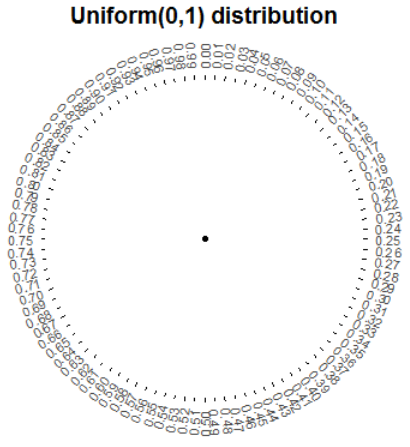
\includegraphics[width=5.69in]{_graphics/uniform-spinner} \caption{A Uniform(0, 1) spinner. The values in the picture are rounded to two decimal places, but in the idealized model the spinner is infinitely precise so that any real number between 0 and 1 is a possible outcome.}\label{fig:uniform-spinner}
\end{figure}

\begin{solution}
\iffalse{} {Solution. } \fi{}
to Example \ref{exm:uniform-outcome}
\end{solution}

An outcome is now a pair of values \((\omega_1, \omega_2\)) corresponding to the results of the first and second spins. The sample space is \(\Omega = [0,1]\times [0,1]\), where \([0,1]\times [0,1]\), also denoted \([0,1]^2\), is the Cartesian product \([0,1]\times [0,1] = \{(\omega_1, \omega_2): \omega_1 \in [0, 1], \omega_2 \in [0, 1]\}\).

In the above (idealized) example, outcomes were measured on a continuous scale; any real number between 0 and 1 was a possible outcome of a single spin (of the idealized, infinitely precise spinner). Even in situations where outcomes are inherently discrete, it is often more convenient to model them as continuous. For example, if an outcome represents the annual salary in dollars of a randomly selected U.S. household, it would be more convenient to model the sample space as the continuous interval\^{}{[}We could also try \([0, m]\) where \(m\) is some large dollar amount providing an upper bound on the maximum possible salary. But we would need to be sure that \(m\) is large enough so that all possible outcomes are in the sample space \([0, m]\). Without knowing this bound in advance, it is convenient to just choose the unbounded interval \([0, \infty)\).{]} \([0, \infty)\) rather than \(\{0, 1, 2, \ldots\}\) or \(\{0, 0.01, 0.02, \ldots\}\).

\begin{example}
\protect\hypertarget{exm:SAT-outcome}{}{\label{exm:SAT-outcome} }Select a U.S. high school student and record the student's SAT Math and Reading score. What is an appropriate sample space?
\end{example}

\begin{solution}
\iffalse{} {Solution. } \fi{}to Example \ref{exm:SAT-outcome}
\end{solution}

An outcome will be an ordered pair represent (Math, Reading) score. Technically, possible scores are 200 through 800 in increments of 10. So we could consider the sample space to be \(\{200, 210, 220, \ldots, 790, 800\}\times \{200, 210, 220, \ldots, 790, 800\}\).

However, we could also model scores on a continuous scale, taking any value in the interval from 200 to 800. In this case, the sample space would be \(\Omega = [200, 800] \times [200, 800]\). Such a specification is often more convenient mathematically.

Add somewhere something like: In practice we rarely enumerate the sample space as we did in the examples in this section. Nonetheless, there is always some underlying sample space corresponding to all possible outcomes of the random phenomenon. Even when we do not specify the sample space, it is important to consider what the sample space is. We must first determine what is possible before determining when is probable. The sample space in essence defines our denominator. Does the sample space corresponding to a single lottery ticket or some lottery ticket somewhere? (Need an example that highlights different denominators of sample space. Maybe like Oscar winner example?)

\hypertarget{events}{%
\section{Events}\label{events}}

In a random phenomenon, an ``event'' is something that could happen. For example, if we're interested in tomorrow's weather, events include

\begin{itemize}
\tightlist
\item
  ``the high temperature is 75°F''
\item
  ``the high temperature is above 75°F''
\item
  ``it rains''
\item
  ``it does not rain''
\item
  ``it rains and the high temperature is above 75°F''
\item
  and so on
\end{itemize}

Mathematically, an \emph{event} is a collection of sample space outcomes that satisfy some criteria.

\begin{definition}
\protect\hypertarget{def:event}{}{\label{def:event} }An \textbf{event} \(A\) is a \emph{subset} of the sample space: \(A\subseteq \Omega\). The collection of all events of interest\footnote{For the purposes of this text, \(\mathcal{F}\) can be considered to be the set of all subsets of \(\Omega\). Technically, \(\mathcal{F}\) is a \emph{\(\sigma\)-field} of subsets of \(\Omega\): \(\mathcal{F}\) contains \(\Omega\) and is closed under countably many elementary set operations (complements, unions, intersections). This requirement ensures that if \(A\) and \(B\) are ``events of interest'', then so are \(A\cup B\), \(A\cap B\), and \(A^c\). While this level of technical detail is not needed, we prefer to introduce the idea of a ``collection of events'' now since a probability measure is a function whose input is an event (set) and not an outcome.} is denoted \(\mathcal{F}\). If the random phenomenon yields outcome \(\omega\), we say ``event \(A\) occurred'' if \(\omega\in A\).
\end{definition}

\begin{itemize}
\tightlist
\item
  Recall that the sample space is the collection of all possible
  outcomes of a random phenomenon.
\item
  An event represents those outcomes which satisfy some criteria.
\item
  There is a single sample space, upon which all events are defined.
\item
  An outcome in a sample space should be defined to record as much information as possible so that the occurrence or non-occurrence of all events of interest can be determined.
\item
  Events are typically denoted with capital letters near the start of the alphabet, with or without subscripts (e.g.~\(A\), \(B\), \(C\), \(A_1\), \(A_2\))
\item
  Events can be composed from others using \href{https://en.wikipedia.org/wiki/Set_(mathematics)\#Basic_operations}{basic set operations} like unions (\(A\cup B\)), intersections (\(A \cap B\)), and complements (\(A^c\)).

  \begin{itemize}
  \tightlist
  \item
    Read \(A^c\) as ``not'' \(A\).
  \item
    Read \(A\cap B\) as ``\(A\) and \(B\)''
  \item
    Read \(A \cup B\) as ``\(A\) or \(B\)''. Note that unions (\(\cup\), ``or'') are always inclusive. \(A\cup B\) occurs if \(A\) occurs but \(B\) does not, \(B\) occurs but \(A\) does not, or both \(A\) and \(B\) occur.
  \end{itemize}
\item
  An event \(A\) is a set. The collection \(\mathcal{F}\) is a \emph{collection of sets}.
\item
  While an event is always a set, it can be a set consisting of a single outcome, or no outcomes at all (the empty set \(\emptyset\)).
\item
  A collection of events \(A_1, A_2, \ldots\) are \textbf{disjoint} (a.k.a. mutually exclusive) if \(A_i \cap A_j = \emptyset\) for all \(i \neq j\). Events are disjoint if they have no outcomes in common.
\end{itemize}

As an example, consider a single roll of a four-sided die. The sample space consists of the four possible outcomes \(\Omega = \{1, 2, 3, 4\}\). Any subset of this sample space is an event. The following table lists he collection of all events (\(\mathcal{F}\)), and whether they occur if the single roll results in a 3 (that is, for the outcome \(\omega=3\)).

\begin{longtable}[]{@{}lll@{}}
\toprule
Event & Description & Occurs upon outcome \(\omega=3\)?\tabularnewline
\midrule
\endhead
\(\emptyset\) & Roll nothing (not possible) & No\tabularnewline
\(\{1\}\) & Roll a 1 & No\tabularnewline
\(\{2\}\) & Roll a 2 & No\tabularnewline
\(\{3\}\) & Roll a 3 & Yes\tabularnewline
\(\{4\}\) & Roll a 4 & No\tabularnewline
\(\{1, 2\}\) & Roll a 1 or a 2 & No\tabularnewline
\(\{1, 3\}\) & Roll a 1 or a 3 & Yes\tabularnewline
\(\{1, 4\}\) & Roll a 1 or a 4 & No\tabularnewline
\(\{2, 3\}\) & Roll a 2 or a 3 & Yes\tabularnewline
\(\{2, 4\}\) & Roll a 2 or a 4 & No\tabularnewline
\(\{3, 4\}\) & Roll a 3 or a 4 & Yes\tabularnewline
\(\{1, 2, 3\}\) & Roll a 1, 2, or 3 (a.k.a. do not roll a 4) & Yes\tabularnewline
\(\{1, 2, 4\}\) & Roll a 1, 2, or 4 (a.k.a. do not roll a 3) & No\tabularnewline
\(\{1, 3, 4\}\) & Roll a 1, 3, or 4 (a.k.a. do not roll a 2) & Yes\tabularnewline
\(\{2, 3, 4\}\) & Roll a 2, 3, or 4 (a.k.a. do not roll a 1) & Yes\tabularnewline
\(\{1, 2, 3, 4\}\) & Roll something & Yes\tabularnewline
\bottomrule
\end{longtable}

\begin{example}
\protect\hypertarget{exm:dice-event}{}{\label{exm:dice-event} }Roll a four-sided die \emph{twice}, and record the result of each roll in sequence. For example, the outcome \((3, 1)\) represents a 3 on the first roll and a 1 on the second; this is not the same outcome as \((1, 3)\).
\end{example}

\begin{enumerate}
\def\labelenumi{\arabic{enumi}.}
\tightlist
\item
  Identify the sample space.
\item
  Identify \(A\), the event that the sum of the two dice is 4.
\item
  Identify \(B\), the event that the sum of the two dice is at most 3.
\item
  The previous events consider the sum of the two dice. Explain why we don't just consider the sample space to be \(\{2, \ldots, 8\}\), so that for example \(B = \{2, 3\}\).
\item
  Identify \(C\), the event that the larger of the two rolls (or the common roll if a tie) is 3
\item
  Identify and interpret \(A\cap C\).
\item
  Identify \(D\), the event that the first roll is a 3.
\item
  Identify \(E\), the event that the second roll is a 3.
\item
  Indetify and interpret \(D \cap E\).
\item
  Identify and interpret \(D \cup E\).
\item
  If the outcome is \((1, 3)\), which of the events above occurred?
\end{enumerate}

\begin{solution}
\iffalse{} {Solution. } \fi{}to Example \ref{exm:dice-event}
\end{solution}

\begin{enumerate}
\def\labelenumi{\arabic{enumi}.}
\tightlist
\item
  The sample space consists of 16 possible ordered pairs of rolls
  \begin{align*}
  \Omega & = \{(1, 1), (1, 2), (1, 3), (1, 4), (2, 1), (2, 2), (2, 3), (2, 4),\\
  & \quad (3, 1), (3, 2), (3, 3), (3, 4), (4, 1), (4, 2), (4, 3), (4, 4)\}
  \end{align*}
\item
  \(A=\{(1, 3), (2, 2), (3, 1)\}\) is the event that the sum of the two dice is 4.
\item
  \(B=\{(1, 1), (1, 2), (2, 1)\}\) is the event that the sum of the two dice is at most 3.
\item
  We might be interested in events other than ones that involve the sum of the dice, like those in the following parts. Knowing just the sum of the dice does not provide enough information to investigate such events.
\item
  \(C=\{(1, 3), (2, 3), (3, 1), (3, 2), (3, 3)\}\), the event that the larger of the two rolls (or the common roll if a tie) is 3
\item
  \(A\cap C=\{(1, 3), (3, 1)\}\) is the event that both the sum of the two dice is 4 and the larger of the two rolls is 3.
\item
  \(D=\{(3, 1), (3, 2), (3, 3), (3, 4)\}\), the event that the first roll is a 3. Note that each outcome in the sample space consists of a pair of rolls, so we must account for both rolls in defining events, even if the event of interest involves just the first roll. There is always a single sample space upon which all events are defined.
\item
  \(E=\{(1, 3), (2, 3), (3, 3), (4, 3)\}\), the event that the second roll is a 3. Note that this is not the same event as \(D\).
\item
  \(D \cap E = \{(3, 3)\}\) is the event that both rolls result in a 3. While an event is always a set, it can be a set consisting of a single outcome (or the empty set).
\item
  \(D \cup E = \{(3, 1), (3, 2), (3, 3), (3, 4), (1, 3), (2, 3), (4, 3)\}\) is the event that at least one of the two rolls results in a 3. Notice that the union is inclusive: \((3, 3)\) is an element of \(D\cup E\). But also notice that the outcome \((3, 3)\) only appears once in the set \(D \cup E\).
\item
  If the outcome is \((1, 3)\) then events \(A\), \(C\), \(A\cap C\), \(E\), \(D\cup E\) all occur. Events \(B\), \(D\), and \(D\cap E\) do not occur.
\end{enumerate}

\begin{example}
\protect\hypertarget{exm:coin-event}{}{\label{exm:coin-event} }Flip a coin 4 times, and record the result of each trial in sequence. For example, HTTH means heads on the first on last trial and tails on the second and third.
\end{example}

\begin{enumerate}
\def\labelenumi{\arabic{enumi}.}
\tightlist
\item
  Specify the sample space.
\item
  Identify \(A\), the event that exactly 3 of the flips land on heads.
\item
  Identify \(B\), the event that exactly 4 of the flips land on heads.
\item
  Identify \(C\), the event that the at least 3 of the flips land on heads. How does \(C\) relate to \(A\) and \(B\)?
\item
  The previous events all consider the number of heads flipped. Explain why we don't just consider the sample space to be \(\{0, 1, 2, 3, 4\}\), so that for example \(C = \{3, 4\}\).
\item
  Identify \(D\), the event that at least 3 heads are flipped in a row.
\item
  Identify \(E\), the event that the first two flips results in tails.
\item
  Identify \(D\cap E\).
\item
  If the outcome is HHTH, which of the events above occurred?
\end{enumerate}

\begin{solution}
\iffalse{} {Solution. } \fi{}to Example \ref{exm:coin-event}
\end{solution}

\begin{enumerate}
\def\labelenumi{\arabic{enumi}.}
\tightlist
\item
  The sample space is composed of 16 outcomes
  \begin{align*}
  \Omega & = \{HHHH, HHHT, HHTH, HTHH, THHH, HHTT, HTHT, HTTH,\\ 
  & \qquad THHT, THTH, TTHH, HTTT, THTT, TTHT, TTTH, TTTT\}
  \end{align*}
\item
  \(A = \{HHHT, HHTH, HTHH, THHH\}\) is the event that exactly 3 of the flips land on heads
\item
  \(B = \{HHHH\}\), the event that exactly 4 of the flips land on heads. While an event is always a set, it can be a set consisting of a single outcome.
\item
  \(C = \{HHHT, HHTH, HTHH, THHH, HHHH\}\) is the event that the at least 3 of the flips land on heads. Also \(C = A \cup B\).
\item
  Yes, the previous events all consider the number of heads flipped, but we might be interested in events --- like the ones in the following parts --- whose occurrence cannot be determined simply by knowing the number of heads. The sample space should always to defined in such a way to provide enough information to investigate any relevant event of interest. There is always a single sample space upon which all events are defined.
\item
  \(D = \{HHHT, THHH, HHHH\}\) is the event that at least 3 heads are flipped in a row. Note that \(D\) is not the same event as \(C\).
\item
  \(E = \{TTHH, TTHT, TTTH, TTTT\}\) is the event that the first two flips result in tails. Note that each outcome consists of the results of 4 flips, so we must account for all 4 flips in defining events. There is always a single sample space upon which all events are defined.
\item
  \(D\cap E=\emptyset\) so the events \(D\) and \(E\) are disjoint; it is not possible to have at least three heads in a row when the first two flips (out of 4) are tails.
\item
  If the outcome is HHTH then events \(A\) and \(C\) occur. Events \(B\), \(D\), \(E\), and \(D \cap E\) do not occur.
\end{enumerate}

\begin{example}[Matching problem]
\protect\hypertarget{exm:matching-event}{}{\label{exm:matching-event} \iffalse (Matching problem) \fi{} }So-called ``matching problems'' concern the following generic scenario. A set of \(n\) cards labeled \(1, 2, \ldots, n\) are placed in \(n\) boxes labeled \(1, 2, \ldots, n\), with exactly one card in each box. Typical questions of interest involve whether the number of a card matches the number of the box in which it is placed. (More colorful descriptions include \href{http://www.rossmanchance.com/applets/randomBabies/RandomBabies.html}{returning babies at random to mothers} or \href{https://fivethirtyeight.com/features/everythings-mixed-up-can-you-sort-it-all-out/}{placing rocks at random back on a museum shelf}.) Consider the case \(n=4\).
\end{example}

\begin{enumerate}
\def\labelenumi{\arabic{enumi}.}
\tightlist
\item
  Identify a reasonable sample space.
\item
  Specify the event that all cards match their box.
\item
  Specify the event that no cards match their box.
\item
  Specify the event that exactly 3 cards match their box.
\item
  Specify the event that card 3 is placed in box 3.
\end{enumerate}

\begin{solution}
\iffalse{} {Solution. } \fi{}to Example \ref{exm:matching-event}
\end{solution}

\begin{enumerate}
\def\labelenumi{\arabic{enumi}.}
\tightlist
\item
  We can consider each outcome to be a particular placement of cards in the boxes. For example, the outcome 3214 (or \((3, 2, 1, 4)\)) represents that card 3 is placed in box 1, card 2 in box 2, card 1 in box 3, and card 4 in box 4. So the sample space consists of the following 24 outcomes\footnote{There are 4 cards that could potentially go in box 1, then 3 cards that could potentially go in box 2, 2 to box 3, and 1 left for box 4. This results in \(4\times3\times2\times1=4! = 24\) possible outcomes. We will see more counting rules in Chapter \ref{counting}}.
  \begin{align*}
  \Omega & = \{1234, 1243, 1324, 1342, 1423, 1432 \\
    & \qquad 2134, 2143, 2314, 2341, 2413, 2431 \\
    & \qquad 3124, 3142, 3214, 3241, 3412, 3421 \\
    & \qquad 4123, 4132, 4213, 4231, 4312, 4321\}
  \end{align*}
\item
  \(A=\{1234\}\) is the event that all cards match their box. While an event is always a set, it can be a set consisting of a single outcome (or the empty set).
\item
  \(B=\{2143, 2341, 2413, 3142, 3412, 3421, 4123, 4312, 4321\}\) is the event that no cards match their box.
\item
  \(\emptyset\) is the event in which exactly 3 cards match their box. There are no outcomes in which exactly 3 cards match; if three cards match, then the fourth card must necessarily match too.
\item
  \(C=\{1234, 1432, 2134, 2431, 4132, 4231\}\) is the event that card 3 is placed in box 3. Since our sample space consists of the placements of each of the cards, each event must be expressed in terms of these outcomes.
\end{enumerate}

Remember that intervals of real numbers such as \((a,b), [a,b], (a,b]\) are also sets, and so can also be events.

\begin{example}
\protect\hypertarget{exm:sat-event}{}{\label{exm:sat-event} }Consider as a sample space all possible scores on the SAT Math exam (ranging from 200 to 800). Even though actual scores are multiples of 10, it is mathematically convenient to consider the sample space as \(\Omega=[200, 800]\), the set of all real numbers between 200 and 800 (rather than \(\{200, 210, 220, \ldots, 800\}\).)
\end{example}
1. Identify \(A\), the event that an SAT Math score is at most 700.
1. Identify \(B\), the event that an SAT Math score is greater than 500.
1. Identify and interpret \(A\cap B\).

\begin{solution}
\iffalse{} {Solution. } \fi{}to Example \ref{exm:sat-event}
\end{solution}

\begin{enumerate}
\def\labelenumi{\arabic{enumi}.}
\tightlist
\item
  \(A=[200, 700]\) is the event that an SAT Math score is at most 700.
\item
  \(B=(500, 800]\) is the event that an SAT Math score is greater than 500.
\item
  \(A\cap B = (500, 700]\) is the event that an SAT Math score is greater than 500 but at most 700.
\end{enumerate}

\begin{example}
\protect\hypertarget{exm:uniform-event}{}{\label{exm:uniform-event} }
Suppose the spinner in Figure \ref{fig:uniform-spinner} is spun twice. Let the sample space be \(\Omega = [0,1]\times [0,1]\). Represent each of the following events using set notation, but also sketch a picture. (Hint: represent the sample space as a square.)
\end{example}

\begin{enumerate}
\def\labelenumi{\arabic{enumi}.}
\tightlist
\item
  Identify \(A\), the event that the first spin is larger then the second.
\item
  Identify \(B\), the event that the smaller of the two spins (or common value if a tie) is less than 0.5.
\item
  Identify \(C\), the event that the sum of the two dice is less than 1.5.
\item
  Identify \(D\), the event that the first spin is less than 0.4.
\end{enumerate}

\begin{solution}
\iffalse{} {Solution. } \fi{}
to Example \ref{exm:uniform-event}
\end{solution}

\begin{enumerate}
\def\labelenumi{\arabic{enumi}.}
\tightlist
\item
  \(A = \{(\omega_1, \omega_2): \omega_1>\omega_2\}\) is the event that the first spin is larger then the second. Note: we only consider \((\omega_1, \omega_2)\) in the sample space \([0, 1]\times[0,1]\); the conditions \(0\le \omega_1 \le 1, 0\le \omega_2 \le 1\) are assumed.\\
\item
  \(B = \{(\omega_1, \omega_2): \min(\omega_1,\omega_2)<0.5\}\) is the event that the smaller of the two spins (or common value if a tie) is less than 0.5. This is equivalent to the event that at least one of the spins is less than 0.5 \(B = \{(\omega_1, \omega_2): \omega_1<0.5 \text{ or } \omega_2<0.5\} = ([0.5, 1]\times[0.5, 1])^c\).
\item
  \(C = \{(\omega_1, \omega_2): \omega_1+\omega_2\ge 1.5\} = \{(\omega_1, \omega_2): \omega_2\ge 1.5-\omega_1\}\) is the event that the sum of the two dice is at least 1.5.
\item
  \(D = \{(\omega_1, \omega_2): \omega_1<0.4\}\) is the event that the first spin is less than 0.4. Remember, sample space outcomes are pairs of spins.
\end{enumerate}



\begin{figure}
\centering
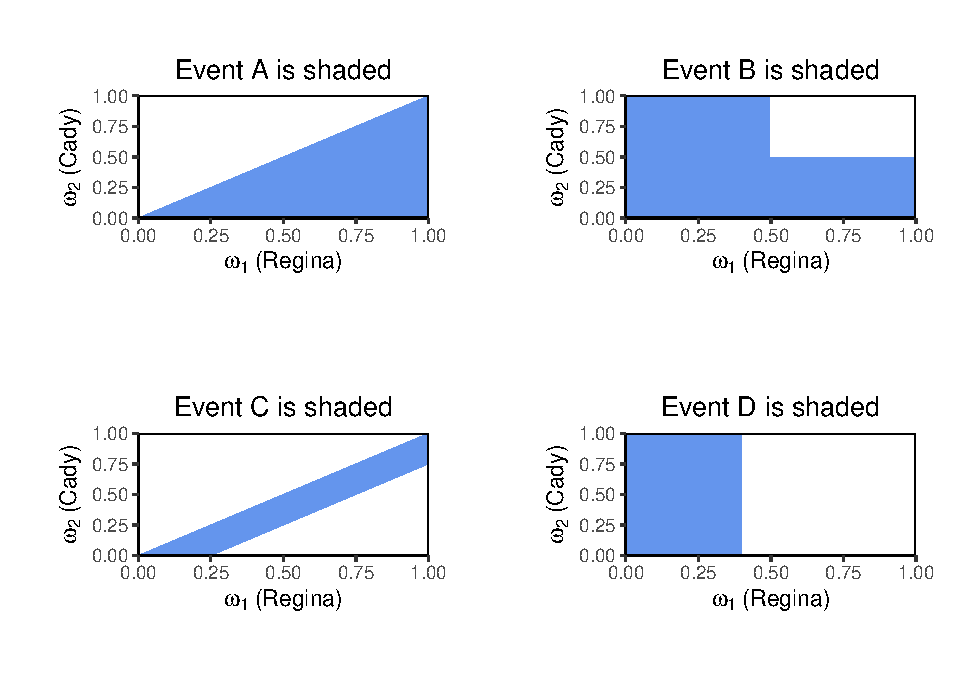
\includegraphics{bookdown-demo_files/figure-latex/uniform-event-plot-1.pdf}
\caption{\label{fig:uniform-event-plot}Illustration of the events in Exercise \ref{exm:uniform-event}. The square represents the sample space \(\Omega=[0,1]\times[0,1]\).}
\end{figure}

\begin{example}[Don't do what Donny Don't does.]
\protect\hypertarget{exm:dd-event}{}{\label{exm:dd-event} \iffalse (Don't do what Donny Don't does.) \fi{} }Donny Don't is asked a series of questions involving a pair of rolls of six-sided dice, such as ``what is the event that the sum of the dice is at least 10''. Donny's responses are below; explain to him what is wrong with his responses and help him see the correct answers.
\end{example}

\begin{enumerate}
\def\labelenumi{\arabic{enumi}.}
\tightlist
\item
  The possible rolls are 1 through 6, so the sample space is \(\{1, 2, 3, 4, 5, 6\}\).
\item
  The sum of the two dice can be 2 through 12, so the event that the sum of the two dice is at least 10 is \(\{10, 11, 12\}\).
\item
  The event that the first roll is a 3 is \(\{3\}\).
\item
  The event that the first roll is a 3 and the second roll is a 1 is \(\{3, 1\}\)
\item
  Donny's sample space from the first question might correspond to what dice rolling scenario? What does \(\{3, 1\}\) represent in this scenario?
\end{enumerate}

\begin{solution}
\iffalse{} {Solution. } \fi{}to Example \ref{exm:dd-event}
\end{solution}

\begin{enumerate}
\def\labelenumi{\arabic{enumi}.}
\tightlist
\item
  The questions involve a pair of rolls, so best to record an outcome as an ordered pair, e.g., (5, 2) for 5 on the first roll and 2 on the second. Therefore, the sample space would be the following set of 36 possible outcomes.
  \begin{align*}
  \Omega  = & \{
  (1, 1), (1, 2), \ldots, (1, 6),\\
  & \;\; (2, 1), (2, 2), \ldots, (2, 6),\\
  & \;\; \vdots\qquad \qquad \quad \cdots \qquad \vdots\\
  & \;\; (6, 1), (6, 2), \ldots, (6, 6)
  \}
  \end{align*}
\item
  Donny's answers to the first two parts are inconsistent, since there is always a single sample space. So if he says the answer to the first part is \(\{1, \ldots, 6\}\), then any event must be a subset of that sample space and his answer to the second part must be wrong. Using the sample space of 36 ordered pairs from the previous answer, the correct event that the sum of the two dice is at least 10 is
  \[
  \{(4, 6), (5, 5), (5, 6), (6, 4), (6, 5), (6, 6)\}
  \]
  If Donny's sample space in the first part had been \(\{2, \ldots, 12\}\), corresponding to the sum of the two dice, then his answer of \(\{10, 11, 12\}\) would have been correct. However, using such a sample space, he would not have been able to answer the remaining questions (which don't involve the sum of the rolls). There is always one sample space on which all events are defined.
\item
  Donny didn't take into account that an outcome is a pair of rolls. The correct event is \(\{(3, 1), (3, 2), (3, 3), (3, 4), (3, 5), (3, 6)\}\), the set of all pairs of rolls for which the first roll is 3.
\item
  Maybe Donny is just using bad notation here, but it sure looks like he is confusing an outcome with an event. The answer should be \(\{(3, 1)\}\), the set containing the single outcome \((3, 1)\). Notice that this is not the same set as \(\{(1, 3)\}\). (But the set \(\{3, 1\}\) is the same as the set \(\{1, 3\}\).)
\item
  The sample space of \(\{1, 2, 3, 4, 5, 6\}\) could correspond to a \emph{single} roll of a fair six-sided die. In this case, the event \(\{3, 1\}\) would be the event that the roll is either a 3 or a 1. (The set \(\{3, 1\}\) is the same as the set \(\{1, 3\}\).)
\end{enumerate}

\begin{example}[Don't do what Donny Don't does.]
\protect\hypertarget{exm:dd-events}{}{\label{exm:dd-events} \iffalse (Don't do what Donny Don't does.) \fi{} }
At various points in his homework, Donny Don't writes the following. Explain to Donny, both mathematically and intuitively, why each of the following symbols is nonsense. Below, \(A\) and \(B\) represent events, \(X\) and \(Y\) represent random variables.
\end{example}

\begin{enumerate}
\def\labelenumi{\arabic{enumi}.}
\tightlist
\item
  \(\IP(A = 0.5)\)
\item
  \(\IP(A + B)\)
\item
  \(\IP(A) \cup \IP(B)\)
\item
  \(\IP(X)\)
\item
  \(\IP(X = A)\)
\item
  \(\IP(X \cap Y)\)
\end{enumerate}

\begin{solution}
\iffalse{} {Solution. } \fi{}to Example \ref{exm:dd-events}
\end{solution}

\begin{enumerate}
\def\labelenumi{\arabic{enumi}.}
\tightlist
\item
  \(A\) is a set and 0.5 is a number; it doesn't make mathematical sense to equate them. Suppose that \(A\) is the event that is rains tomorrow. It doesn't make sense to say (as \(A=1\) does) ``it rains tomorrow equals 0.5''. If we want to say ``the probability that it rains tomorrow equals 0.5'' we should write \(\IP(A) = 0.5\).
\item
  \(A\) and \(B\) are sets; it doesn't make mathematical sense to add them. Suppose that \(B\) is the event that tomorrow's high temperature is above 80 degrees F. It doesn't make sense to say (as \(A+B\) does) ``the sum of (it rains tomorrow) and (tomorrow's high temperature is above 80 degrees F)''. If we want ``(it rains tomorrow) OR (tomorrow's high temperature is above 80 degrees F)'', then we need \(A\cup B\). Union is an operation on sets; addition is an operation on numbers.
\item
  \(\IP(A)\) and \(\IP(B)\) are numbers; union is an operation on sets, it doesn't make mathematical sense to take a union of numbers. Since \(\IP(A)\) and \(\IP(B)\) are numbers then mathematically we can add them. But keep in mind that \(\IP(A)+\IP(B)\) is not necessarily a probability, for example if \(\IP(A)=0.5\) and \(\IP(B)=0.6\). If we want ``the probability that (it rains tomorrow) OR (tomorrow's high temperature is above 80 degrees F)'' then the correct symbol is \(\IP(A\cup B)\), which would be equal to \(\IP(A)+\IP(B)\) only if \(A\) and \(B\) were disjoint (which in the example would mean it's not possible to have a rainy day with a high temperature above 80 degrees F).
\item
  \(X\) is a random variable, and probabilities are assigned to events. If \(X\) is tomorrow's high temperature in degrees F then \(P(X)\) reads ``the probability that tomorrow's high temperature in degrees F'', which is missing any qualifying information that could define an event. We could write \(\IP(X>80)\) to represent ``the probability that (tomorrow's high temperature is greater than 80 degrees F)''.
\item
  \(X\) is a random variable (a function) and \(A\) is an event (a set), and it doesn't make sense to equate these two different mathematical objects. It doesn't make sense to say (as \(X=A\) does) ``tomorrow's high temperature in degrees F equals the event that it rains tomorrow''.
\item
  \(X\) and \(Y\) are RVs (functions) and intersection is an operation on sets. If \(Y\) is the amount of rainfall in inches tomorrow then \(X \cap Y\) is attempting to say ``tomorrow's high temperature in degrees F and the amount of rainfall in inches tomorrow'', but this is still missing qualifying information to define a valid event for which a probability can be assigned. We could say \(\IP(\{X > 80\} \cap \{Y < 2\})\) to represent ``the probability that (tomorrow's high temperature is greater than 80 degrees F) AND (the amount of rainfall tomorrow is less than 2 inches)''.
\end{enumerate}

\hypertarget{rv}{%
\section{Random variables}\label{rv}}

Statisticians use the terms \emph{observational unit} and \emph{variable}. Observational units are the people, places, things, etc., for which data are observed. Variables are the measurements made on the observational units. For example, the observational units in a study could be college students, while variables could be high school GPA, college GPA, SAT score, years in college, number of Statistics courses taken, etc.

In probability, an \emph{outcome} of a random phenomenon plays a role analogous to an observational unit in statistics. The sample space of outcomes is often only vaguely defined. In many situations we are less interested in detailing the outcomes themselves and more interested in whether or not certain events occur, or with measurements that we can make for the outcomes. For example, if the random phenomenon corresponds to randomly selecting a random sample of students at a college, an outcome could be the list of students selected for the sample. But we are less interested in who the students are, and more interested in questions which involve variables, such as: what is the distribution of SAT scores? What is the relationship between high school GPA and college GPA? What is the average number of years before graduation?

Roughly, a \emph{random variable} assigns a number to each outcome of a random phenomenon. More precisely

\begin{definition}
\protect\hypertarget{def:rv}{}{\label{def:rv} }
A \textbf{random variable (RV)} \(X\) is a \emph{function} that takes an outcome in the sample space as input and returns a real number as output; that is, \(X:\Omega \mapsto \mathbb{R}\). Random variables are typically denoted by capital letters near the end
of the alphabet, with or without subscripts: e.g.~\(X\), \(Y\), \(Z\), or \(X_1\), \(X_2\), \(X_3\), etc. The value that the random variable \(X\) assigns to the outcome \(\omega\) is denoted \(X(\omega)\).
\end{definition}

\begin{example}
\protect\hypertarget{exm:coin-rv}{}{\label{exm:coin-rv} }
Flip a coin 4 times, and record the result of each trial in sequence. For example, HTTH means heads on the first on last trial and tails on the second and third. One random variable is \(X\), the number of heads flipped.
\end{example}

\begin{enumerate}
\def\labelenumi{\arabic{enumi}.}
\tightlist
\item
  Explain why \(X\) is a random variable.
\item
  Evaluate each of the following: \(X(HHHH), X(HTHT), X(TTHH)\).
\item
  Identify the possible values of \(X\). Why not let the sample space just consist of this set of possible values?
\end{enumerate}

\begin{solution}
\iffalse{} {Solution. } \fi{}to Example \ref{exm:coin-rv}
\end{solution}

\begin{enumerate}
\def\labelenumi{\arabic{enumi}.}
\tightlist
\item
  \(X\) maps each outcome to a number via the function ``count the number of heads''.
\item
  \(X(HHHH) = 4, X(HTHT) = 2, X(TTHH) = 2\).
\item
  The possible values of \(X\) are \(0, 1, 2, 3, 4\). You might ask: if we only care about the number of heads, why bother with the coin flip sequence at all? That is, why not define the sample space as \(\{0, 1, 2, 3, 4\}\) rather than \(\{HHHH, HHHT, HHTH, \ldots\}\). The main reason why is that we often want to define many random variables on the same sample space, and study the relationships between random variables. For example, if a sample space outcome were just the number of heads, we would not be able to obtain information about the longest number of heads in a row, or the proportion of heads on trials that follow heads. Moreover we would not be able to study the relationship between random variables unless they were defined on a common sample space. As a statistics analogy, you would not be able to study the relationship between SAT scores and college GPA unless you measured both variables for the same set of observational units. (Another but less important reason is that is often convenient to work with probability spaces in which the outcomes are equally likely, as is the case for \(\{HHHH, HHHT, HHTH, \ldots\}\) but not for \(\{0, 1, 2, 3, 4\}\), for four flips of a fair coin.)
\end{enumerate}

The RV itself is typically denoted with a capital letter (\(X\)); possible values of that
random variable are denoted with lower case letters (\(x\)). Think of the capital letter \(X\) as a label standing in for a formula like ``the number of heads in 4 flips of a coin'' and \(x\) as a dummy variable
standing in for a particular value like 3.

We are often interested in events which involve random variables. For example, the expressions \(X=x\) or \(\{X=x\}\) are shorthand for the \emph{event} \(\{\omega\in\Omega: X(\omega)=x\}\), the set of outcomes \(\omega\) for which \(X(\omega)=x\). Remember that any event is a subset of the \emph{sample space}. So objects like \(\{X=x\}\) are subsets\footnote{Technically, we have some collection \(\mathcal{F}\) of events of interest, and so we require sets like \(\{X\le x\}\) to be in \(\mathcal{F}\). This requirement is satified by requiring \(X\) to be an \emph{\(\mathcal{F}\)-measurable} function.} of \(\Omega\).

\begin{example}
\protect\hypertarget{exm:coin-rv-event}{}{\label{exm:coin-rv-event} }Flip a coin 4 times, and record the result of each trial in sequence. For example, HTTH means heads on the first on last trial and tails on the second and third. One random variable is \(X\), the number of heads flipped.
\end{example}

\begin{enumerate}
\def\labelenumi{\arabic{enumi}.}
\tightlist
\item
  Identify and interpret the event \(\{X=3\}\). That is, identify the outcomes \(\omega\) for which \(X(\omega)=3\).
\item
  Identify and interpret the event \(\{X=4\}\).
\item
  Identify and interpret the event \(\{X\ge3\}\). How is this event related to the previous two?
\end{enumerate}

\begin{solution}
\iffalse{} {Solution. } \fi{}to Example \ref{exm:coin-rv-event}
\end{solution}

\begin{enumerate}
\def\labelenumi{\arabic{enumi}.}
\tightlist
\item
  \(\{X=3\} = \{HHHT, HHTH, HTHH, THHH\}\) is the event that exactly 3 of the flips land on heads. This is an event because it is a subset of the sample space.
\item
  \(\{X=4\}= \{HHHH\}\), the event that exactly 4 of the flips land on heads. Notice that the event is the set \(\{HHHH\}\), which consists of the single outcome \(HHHH\).
\item
  \(\{X\ge3\} = \{HHHT, HHTH, HTHH, THHH, HHHH\}\) is the event that the at least 3 of the flips land on heads. Also \(\{X\ge 3\} = \{X=3\}\cup \{X=4\}\).
\end{enumerate}

Recall that for a mathematical function\footnote{Throughout, we use \(g\) to denote a generic function, and reserve \(f\) to represent a probability density function. Likewise, we represent a generic function argument (or ``dummy variable'') with \(u\), since \(x\) is often used to represent possible values of a random variable \(X\); in the RV scenario \(x\) typically represents the \emph{output} of the function \(X\) rather than the input (which is a sample space outcome \(\omega\).)} \(g\), given an input \(u\), the function returns a real number \(g(u)\). For example, if \(g(u) = u^2\) then \(g(3) = 9\). If the input comes from some set \(S\) (i.e.~\(u\in S\)), we often write \(g:S\mapsto \mathbb{R}\).

Likewise, a random variable \(X\) is a function which maps each outcome \(\omega\) in the sample space \(\Omega\) to a real number \(X(\omega)\); \(X:\Omega\mapsto\mathbb{R}\). For a single outcome \(\omega\), the value \(x = X(\omega)\) is a single number; notice that \(x\) represents the \emph{output} of the function \(X\) rather than the input. However, it is important to remember that the RV \(X\) itself is a \emph{function}, and \emph{not} a single number.

You are probably familiar with functions which have simple closed form formulas of their arguments: \(g(u)=5u\), \(g(u)=u^2\), \(g(u)=e^u\), etc. While any random variable is some function, the function is rarely specified as an explicit mathetical formula of its input \(\omega\). Often, outcomes are not even numbers (e.g., sequences of coin flips), or only vaguely specified if at all (e.g., possible paths of a hurricane). In the coin flip example, we defined \(X\) only through the words ``number of flips that land on heads''; translating even this simple situation into a formula of \(\omega\) requires some notation\footnote{It's easiest if we label a flip of heads as 1 and tails as 0. Represent an outcome \(\omega\) as \((\omega_1, \omega_2, \omega_3, \omega_4)\), where \(\omega_i\in\{0,1\}\) is the result of the \(i\)th flip. Then \(X(\omega)=\sum_{i=1}^{4} \omega_i\) represents the number of heads. For example, outcome HHTH would be represented as \((1, 1, 0, 1)\) and \(X((1, 1, 0, 1)) = 1 + 1 + 0 + 1 = 3\). This could be coded as \texttt{sum(omega)}.}.

It is more appropriate to think of a RV as a function in the sense of a scale at a grocery store which maps a fruit to its weight, \(X: \text{fruit}\mapsto\text{weight}\). Put an apple on the scale and the scale returns a number, \(X(\text{apple})\), the weight of the apple. Likewise, \(X(\text{orange})\), \(X(\text{banana})\). The RV \(X\) is the scale itself. (This simplistic analogy assumes a sample space outcome is a single fruit. Of course, it's even more complicated in reality since an outcome can be considered a set of fruits, so that we have for example \(X(\{\text{2 apples}, \text{3 oranges}\})\), and all fruits do not weigh the same, so that \(X(\text{this apple})\) is not the same as \(X(\text{that apple})\).)

The RV itself is denoted with a capital letter; possible values of that
random variable are denoted with lower case letters. For example \(\{X=x\}\) is shorthand for the event \(\{\omega\in\Omega: X(\omega)=x\}\), the set of outcomes \(\omega\) for which \(X(\omega)=x\). Think of the capital letter \(X\) as a label standing in for a formula like ``the number of heads in 4 flips of a coin'' and \(x\) as a dummy variable
standing in for a particular value like 3. Remember that any event is a subset of the \emph{sample space}. So objects like \(\{X=x\}\) are subsets\footnote{Technically, we have some collection \(\mathcal{F}\) of events of interest, and so we require sets like \(\{X\le x\}\) to be in \(\mathcal{F}\). This requirement is satified by requiring \(X\) to be an \emph{\(\mathcal{F}\)-measurable} function.} of \(\Omega\). In the scale analogy if \(X\) is weight measured in pounds, we might have \(\{X>5\}=\{\text{watermelon}, \text{pineapple}\}\) is the set of fruits that weigh more than 5 pounds.

\begin{example}
\protect\hypertarget{exm:dice-rv}{}{\label{exm:dice-rv} }Roll a four-sided die twice, and record the result of each roll in sequence. For example, the outcome \((3, 1)\) represents a 3 on the first roll and a 1 on the second; this is not the same outcome as \((1, 3)\). Let \(X\) be the sum of the two dice, and let \(Y\) be the larger of the two rolls (or the common value if both rolls are the same).
\end{example}

\begin{enumerate}
\def\labelenumi{\arabic{enumi}.}
\tightlist
\item
  Evaluate \(X((1, 3))\), \(X((4, 3))\), and \(X((2,2))\).
\item
  Evaluate \(Y((1, 3))\), \(Y((4, 3))\), and \(Y((2,2))\).
\item
  Identify and interpret \(\{X = 4\}\).
\item
  Identify and interpret \(\{X = 3\}\).
\item
  Identify and interpret \(\{X \le 3\}\).
\item
  Identify and interpret \(\{Y = 4\}\).
\item
  Identify and interpret \(\{Y = 3\}\).
\item
  Identify and interpret \(\{Y \le 3\}\).
\item
  Identify and interpret \(\{X = 4, Y = 3\}\) (that is, \(\{X = 4\}\cap \{Y = 3\}\)).
\item
  Identify and interpret \(\{X = 4, Y \le 3\}\).
\item
  Identify and interpret \(\{X = 3, Y = 3\}\).
\item
  Identify and interpret \(\{X \ge Y\}\).
\item
  Identify the possible values of \(X\).
\item
  Identify the possible values of \(Y\).
\item
  Identify the possible values of the pair \((X, Y)\).
\end{enumerate}

\begin{solution}
\iffalse{} {Solution. } \fi{}to Example \ref{exm:dice-rv}
\end{solution}

\begin{enumerate}
\def\labelenumi{\arabic{enumi}.}
\tightlist
\item
  \(X\) is the sum of the two rolls, so \(X((1, 3))=4\), \(X((4, 3))=7\), and \(X((2,2))=4\).
\item
  \(Y\) is the larger of the two rolls (or the common value if a tie) so \(Y((1, 3))=3\), \(Y((4, 3))=4\), and \(Y((2,2))=2\).
\item
  \(\{X = 4\} =\{(1, 3), (2, 2), (3, 1)\}\) is the event that the sum of the two dice is 4.
\item
  \(\{X = 3\} =\{(1, 2), (2, 1)\}\) is the event that the sum of the two dice is 3.
\item
  \(\{X \le 3\}=\{(1, 1), (1, 2), (2, 1)\}\) is the event that the sum of the two dice is at most 3.
\item
  \(\{Y = 4\}=\{(1, 4), (2, 4), (3, 4), (4, 4), (4, 1), (4, 2), (4,3)\}\) is the event that the larger of the two rolls is 4.
\item
  \(\{Y = 3\}=\{(1, 3), (2, 3), (3, 3), (3, 1), (3, 2)\}\) is the event that the larger of the two rolls is 3.
\item
  \(\{Y \le 3\}=\{(1, 1), (1, 2), (1, 3), (2, 1), (2, 2), (2, 3), (3, 1), (3, 2), (3, 3)\}\) is the event that the larger of the two rolls is at most 3. Notice that since in this example \(Y\) can only take values 1, 2, 3, 4, we have \(\{Y\le 3\} = \{Y=4\}^c\).
\item
  \(\{X = 4, Y = 3\} \equiv \{X = 4\}\cap \{Y = 3\}=\{(1, 3), (3, 1)\}\) is the event that both the sum of the two dice is 4 and the larger of the two rolls is 3. Even though this involves two random variables, it is a single event (that is, a single subset of the sample space). There are only two outcomes for which both the sum of the two dice is 4 and the larger of the two dice is 3.
\item
  \(\{X = 4, Y \le 3\} \equiv \{X = 4\}\cap \{Y \le 3\}=\{(1, 3), (2, 2), (3, 1)\}\) is the event that both the sum of the two dice is 4 and the larger of the two rolls is at most 3. Notice that since in this example \(\{X=4\} \subset \{Y\le 3\}\), we have \(\{X = 4, Y \le 3\} = \{X=4\}\).
\item
  \(\{X = 3, Y = 3\} \equiv \{X = 3\}\cap \{Y = 3\}=\emptyset\), since there are no outcomes for which both the sum is 3 and the larger of the two dice is 3. (If the the larger of the two dice is 3, then the sum must be at least 4.)
\item
  The event \(\{X\ge Y\}\) represents the set of outcomes \(\{\omega: X(\omega) \ge Y(\omega)\}\). In this example, for every possible outcome the sum of the two dice is at least as large as the larger of the two die, so \(\{X \ge Y\} = \Omega\).
\item
  The possible values of \(X\) are \(\{2, 3, \ldots, 8\}\)
\item
  The possible values of \(Y\) are \(\{1, 2, 3, 4\}\)
\item
  The possible values of the pair \((X, Y)\) are \(\{(2, 1), (3, 2), (4, 2), (4, 3), (5, 3), (5, 4), (6, 3), (6, 4), (7, 4), (8,4)\}\). Notice that while, for example, 8 is a possible value of \(X\) and 1 is a possible value of \(Y\), (8, 1) is not a possible value of the pair \((X, Y)\); it's not possible for the larger of the two dice to be 1 but their sum to be 8.
\end{enumerate}

When dealing with probabilities, it is common to write \(\IP(X=3)\) instead of \(\IP(\{X=3\})\), and \(\IP(X = 4, Y = 3)\) instead of \(\IP(\{X = 4\}\cap \{Y = 3\})\); read the comma in \(\IP(X = 4, Y = 3)\) as ``and''. But keep in mind that an expression like ``\(X=3\)'' really represents an event \(\{X=3\}\), an expression which itself represents \(\{\omega\in\Omega: X(\omega) = 3\}\), a subset of \(\Omega\).

\begin{example}
\protect\hypertarget{exm:PP-rv}{}{\label{exm:PP-rv} }
Customers enter a deli and take a number to mark their place in line. When the deli opens the counter starts 0; the first customer to arrive takes number 1, the second 2, etc. We record the counter over time, continuously, as it changes as customers arrive. Time is measured in minutes after the deli opens (time 0). A sample space outcome could be represented as a path of the number of customers over time; a few such paths are illustrated in Figure \ref{fig:coin-sim2}. Notice the stairstep feature: a customer arrives and takes a number then the counter stays on that number for some time (the flat spots) until another customer arrives and the counter increases by one (the jumps).

There are many random variables that could be interest, including

\begin{itemize}
\tightlist
\item
  \(N_t\), the number of customers that have arrived by time \(t\), where \(t\ge0\) is minutes after time 0
\item
  \(T_j\), the time (in minutes after time 0) at which the \(j\)th customer arrives, for \(j=1, 2, \ldots\)
\item
  \(W_j\), the ``waiting'' time (in minutes) between the arrival of the \(j\)th and the \((j-1)\)th customer.
\end{itemize}
\end{example}



\begin{figure}
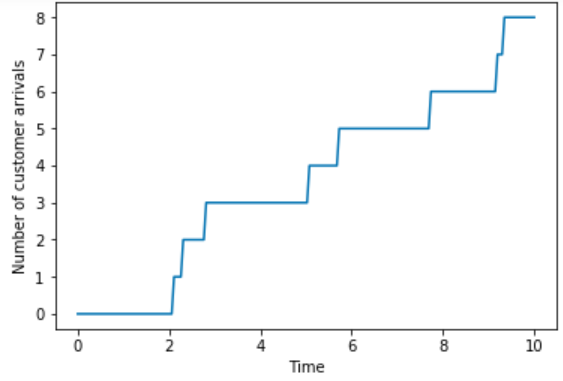
\includegraphics[width=0.5\linewidth]{_graphics/PP-path-one} 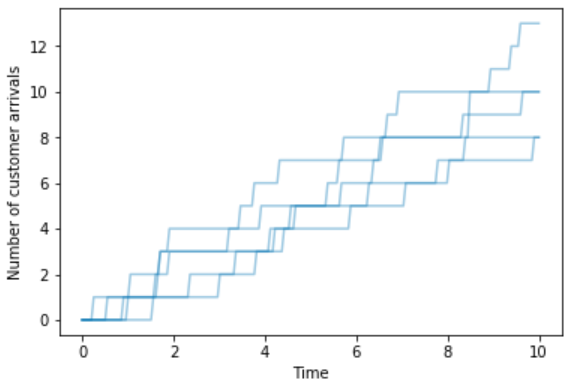
\includegraphics[width=0.5\linewidth]{_graphics/PP-path-several} \caption{Sample space outcomes for Example \ref{exm:PP-rv}. Left: a single sample path of the number of customer arrivals over time. Right: several possible paths.}\label{fig:PP-rv-plot}
\end{figure}

For the outcome represented by the path in the plot on the left in Figure \ref{fig:PP-rv-plot}, identify (as best as you can from the plot) the value of the following random variables.

\begin{enumerate}
\def\labelenumi{\arabic{enumi}.}
\tightlist
\item
  \(N_4\)
\item
  \(N_{6.5}\)
\item
  \(T_4\)
\item
  \(T_5\)
\item
  \(W_1\)
\item
  \(W_5\)
\end{enumerate}

\begin{solution}
\iffalse{} {Solution. } \fi{}to Example \ref{exm:PP-rv}
\end{solution}

\begin{enumerate}
\def\labelenumi{\arabic{enumi}.}
\tightlist
\item
  For this outcome \(N_4=3\); the number of customers that have arrived by time 4 is 3.
\item
  For this outcome \(N_{6.5}=5\); the number of customers that have arrived by time 6.5 is 5. The number of customers is a whole number, but time is measured continuously (e.g., 6.5 minutes after opening).
\item
  For this outcome \(T_4\approx 5.1\). The path jumps to 4 a little after time 5, so the time at which the fourth customer arrives (when the counter jumps to 4) is about 5.1 minutes after open.
\item
  For this outcome \(T_5\approx 5.9\). The path jumps to 5 a little before time 6, so the time at which the fifth customer arrives (when the counter jumps to 5) is about 5.9 minutes after open.
\item
  For this outcome \(W_1\approx 2\). \(W_1\) is the waiting time from open until the first customer arrives, which seems to happen at about time 2 (when the counter jumps to 1).
\item
  For this outcome \(W_5\approx 0.8\). \(W_5\) is the time elapsed between the arrival of the fourth (at time 5.1) and fifth (at time 5.9) customers, which is about 0.8 minutes.
\end{enumerate}

\begin{example}[Matching problem]
\protect\hypertarget{exm:matching-rv}{}{\label{exm:matching-rv} \iffalse (Matching problem) \fi{} }So-called ``matching problems'' concern the following generic scenario. A set of \(n\) cards labeled \(1, 2, \ldots, n\) are placed in \(n\) boxes labeled \(1, 2, \ldots, n\), with exactly one card in each box. Typical questions of interest involve whether the number of a card matches the number of the box in which it is placed. (More colorful descriptions include \href{http://www.rossmanchance.com/applets/randomBabies/RandomBabies.html}{returning babies at random to mothers} or \href{https://fivethirtyeight.com/features/everythings-mixed-up-can-you-sort-it-all-out/}{placing rocks at random back on a museum shelf}.) Consider the case \(n=4\). Let \(Y\) be the number of cards (out of 4) which match the number of the box in which they are placed. For \(j=1, 2, 3, 4\), let \(I_j=1\) if card \(j\) is placed in box \(j\), and let \(I_j=0\) otherwise.
\end{example}

\begin{enumerate}
\def\labelenumi{\arabic{enumi}.}
\tightlist
\item
  Evaluate \(Y(1234)\), \(Y(1243)\), and \(Y(2143)\).
\item
  Evaluate \(I_1(1234)\), \(I_1(1243)\), and \(I_1(2143)\).
\item
  Evaluate \(I_2(1234)\), \(I_2(1243)\), and \(I_2(2143)\).
\item
  Evaluate \(I_3(1234)\), \(I_3(1243)\), and \(I_3(2143)\).
\item
  Evaluate \(I_4(1234)\), \(I_4(1243)\), and \(I_4(2143)\).
\item
  Identify and interpret \(\{Y=4\}\).
\item
  Identify and interpret \(\{Y=0\}\).
\item
  Identify and interpret \(\{Y=3\}\).
\item
  Identify and interpret \(\{I_1=1\}\).
\item
  Identify and interpret \(\{I_3=1\}\).
\item
  What is the relationship between \(Y\) and the \(I_j\)'s?
\end{enumerate}

\begin{solution}
\iffalse{} {Solution. } \fi{}to Example \ref{exm:matching-rv}
\end{solution}

\begin{enumerate}
\def\labelenumi{\arabic{enumi}.}
\tightlist
\item
  \(Y\) counts the number of matches so \(Y(1234)=4\) (all numbers match), \(Y(1243)=2\) (1 and 2 match, 3 and 4 do not), and \(Y(2143)=0\) (no numbers match).
\item
  \(I_1=1\) only if card 1 is in the first position, so \(I_1(1234)=1\), \(I_1(1243)=1\), and \(I_1(2143)=0\).
\item
  \(I_2=1\) only if card 2 is in the second position, so \(I_2(1234)=1\), \(I_2(1243)=1\), and \(I_2(2143)=0\).
\item
  \(I_3=1\) only if card 3 is in the third position, so \(I_3(1234)=1\), \(I_3(1243)=0\), and \(I_3(2143)=0\).
\item
  \(I_4=1\) only if card 4 is in the fourth position, so \(I_4(1234)=1\), \(I_4(1243)=0\), and \(I_4(2143)=0\).
\item
  \(\{Y=4\}=\{1234\}\) is the event that all 4 cards match. Notice that the event is the set \(\{1234\}\), which consists of the single outcome \(1234\).
\item
  \(\{Y=0\}=\{2143, 2341, 2413, 3142, 3412, 3421, 4123, 4312, 4321\}\) is the event that none of the cards match
\item
  \(\{Y=3\}=\emptyset\) is the event in which exactly 3 cards match their box. There are no outcomes in which exactly 3 cards match; if three cards match, then the fourth card must necessarily match too.
\item
  \(\{I_1=1\}=\{1234, 1243, 1324, 1342, 1423, 1432\}\) is the event that card 1 is placed in box 1. Since our sample space consists of the placements of each of the cards, each event must be expressed in terms of these outcomes.
\item
  \(\{I_3=1\}=\{1234, 1432, 2134, 2431, 4132, 4231\}\) is the event that card 3 is placed in box 3. Since our sample space consists of the placements of each of the cards, each event must be expressed in terms of these outcomes.
\item
  \(Y=I_1+I_2+I_3+I_4\). \(Y\) represents the total count of matches. The sum \(I_1+I_2+I_3+I_4\) starts with the first box and adds 1 to the count if there is a match (and 0 otherwise), and continues for each of the boxes, resulting in the total count of matches. For example, \(Y(1243) = 2 = 1 + 1 + 0 + 0 = I_1(1243)+I_2(1243)+I_3(1243)+I_4(1243)\). Notice that all the random variables are defined on the same probability space; that is, they have the same inputs. We expand on this idea further in the next subsection.
\end{enumerate}

Random variables that only take two possible values, 0 and 1, (like \(I_1\) in the previous example) have a special name.

\begin{definition}
\protect\hypertarget{def:indicator}{}{\label{def:indicator} }An \textbf{indicator (a.k.a.~Bernoulli)} RV can take only the values 0 or 1. If \(A\) is an event then the indicator RV \(\ind_A\) is defined as
\[
\ind_A(\omega) =
\begin{cases}
1, & \omega \in A,\\
0, & \omega \notin A
\end{cases}
\]
\end{definition}

That is, \(\ind_A\) equals 1 if event \(A\) occurs, and \(\ind_A\) equals 0 if event \(A\) does not occur. Indicators provide the bridge between events and random variables. While simple, they can are very useful.
For example, representing a count as a sum of indicator RVs as in Exercise \ref{exm:matching-rv} is a very common and useful strategy.

\hypertarget{transform}{%
\subsection{Transformations of random variables}\label{transform}}

\textbf{A function of a random variable is also a random variable.} That is, if \(X\) is a random variable and \(g:\mathbb{R}\mapsto\mathbb{R}\) is a function, then \(Y=g(X)\) is a random variable\footnote{\(Y(\omega) = g(X(\omega))\) so \(Y\) maps \(\Omega\) to \(\mathbb{R}\) via the composition of the functions \(g\) and \(X\); that is, \(Y=g\circ X\)}.

For example, suppose a sample space consists of a set of circles of various sizes. If \(X\) is a random variable representing the radius of a circle selected from this sample space, then \(Y = \pi X^2\) is a random variable representing the area of a circle selected from this sample space. Here we can write \(Y=g(X)\) with \(g(u) = \pi u^2\).

\textbf{Sums and products, etc., of random variables \emph{defined on the same probability space} are random variables.} That is, if random variables \(X\) and \(Y\) are defined on the same probability space then \(X+Y\), \(X-Y\), \(XY\), and \(X/Y\) are also random variables. Similarly, it is possible to make comparisons such as \(X\ge Y\) for random variables defined on the same probability space. The following example emphasizes what we mean be ``defined on the same probability space''.

\begin{example}
\protect\hypertarget{exm:dice-add}{}{\label{exm:dice-add} }Roll a four-sided die twice, and record the result of each roll in sequence. For example, the outcome \((3, 1)\) represents a 3 on the first roll and a 1 on the second; this is not the same outcome as \((1, 3)\). Let \(X_1\) be the result of the first roll, and \(X_2\) the result of the second.
\end{example}

\begin{enumerate}
\def\labelenumi{\arabic{enumi}.}
\tightlist
\item
  Evaluate \(X_1((3, 1))\) and \(X_2((3,1))\).
\item
  If an outcome is represented by \(\omega=(\omega_1, \omega_2)\) (e.g.~(3, 1)), specify the functions that define the random variables \(X_1\) and \(X_2\).
\item
  Is \(X=X_1 + X_2\) a valid random variable? If so, identify the function that defines it.
\item
  Evaluate \(X((3, 1))\).
\end{enumerate}

\begin{solution}
\iffalse{} {Solution. } \fi{}to Example \ref{exm:dice-add}
\end{solution}

\begin{enumerate}
\def\labelenumi{\arabic{enumi}.}
\tightlist
\item
  \(X_1((3, 1))=3\) and \(X_2((3,1))=1\).
\item
  Recall that there is a single sample space corresponding to the pairs of rolls, rather than a separate sample space for each of the individual rolls. Therefore, random variables need to be defined on the sample space corresponding to pairs of rolls. \(X_1((\omega_1, \omega_2))=\omega_1\) and \(X_2((\omega_1, \omega_2))=\omega_2\). That is, \(X_1\) maps an ordered pair to its first coordinate, and \(X_2\) to its second.
\item
  Yes, \(X=X_1 + X_2\) is a valid random variable. For each outcome \((\omega_1, \omega_2)\), \(X\) returns a number: \(X((\omega_1, \omega_2))=X_1((\omega_1, \omega_2)) + X_2((\omega_1, \omega_2))=\omega_1+\omega_2\)
\item
  \(X((3, 1)) = X_1((3, 1))+X_2((3,1))=3+1=4\).
\end{enumerate}

The above example probably seems like notational overkill. And of course we could have defined \(X\) directly as \(X((\omega_1,\omega_2))=\omega_1+\omega_2\) without the need for \(X_1, X_2\). But we introduced the example to emphasize that it only makes sense to add random variables if they are defined on the same sample space. Remember that adding two random variables involves adding two \emph{functions}, in the way that the function \(g = g_1 + g_2\) is defined by \(g(u) = g_1(u) + g_2(u)\). It only makes sense to add two functions together if they have the same inputs.

For example, consider the random variable \(X\) from Example \ref{exm:coin-rv} and the random variable \(Y\) from
Example \ref{exm:matching-rv}. It wouldn't make much practical sense to consider \(X+Y\), but it would make no mathematical sense. How would \(X+Y\) even be defined? \(X\) is defined for sequences of coin flips like HHTH, while \(Y\) is defined for the shuffles in the matching problem like 2143. If you attempted to add \(X\) and \(Y\), which outcomes would go together? Would you add \(X(HHTH)\) to \(Y(2143)\)? Why not add \(X(HHTH)\) to \(Y(1234)\)? Again, adding two random variables involves adding two functions, and it doesn't make sense to add those functions if they have different inputs.

As a more practical example, if \(X\) represents SAT math score and \(Y\) represents SAT verbal score then we might be interested in the total score \(X+Y\). Requiring \(X\) and \(Y\) to be defined on the same probability space is like requiring the scores to be measured for the same students. For example, Antwan has both a Math score \(X(\text{Antwan})\) and a Verbal score \(Y(\text{Antwan})\), so we can consider the total score \((X+Y)(\text{Antwan}) = X(\text{Antwan})+Y(\text{Antwan})\). (In statistical terms, the variables are measured for the same observational units.) It wouldn't make sense to add SAT Math scores from one set of students to SAT verbal scores for a different set of students; for example \(X(\text{Antwan}) + Y(\text{Maria})\) makes no sense.

\begin{example}
\protect\hypertarget{exm:mscoin-rv}{}{\label{exm:mscoin-rv} }
Flip a fair coin four times and record the results in order, e.g.~HHTT means two heads followed by two tails. Recall that in Section \ref{sim} we considered the \emph{proportion of the flips which immediately follow a H that result in H}. Remember that we do not consider this proportion if no flips follow a H, i.e.~the outcome is either TTTT or TTTH.

Let:

\begin{itemize}
\tightlist
\item
  \(Z\) be the number of flips immediately following H.
\item
  \(Y\) be the number of flips immediately following H that result in H.
\item
  \(X\) be the proportion of flips immediately following H that result in H.
\end{itemize}
\end{example}

\begin{enumerate}
\def\labelenumi{\arabic{enumi}.}
\tightlist
\item
  Is \(X\) a random variable? How does it relate to \(Y\) and \(Z\)?
\item
  For each of the possible outcomes in the sample space, find the value of \((Z, Y, X)\).
\end{enumerate}

\begin{solution}
\iffalse{} {Solution. } \fi{}to Example \ref{exm:mscoin-rv}
\end{solution}

\begin{enumerate}
\def\labelenumi{\arabic{enumi}.}
\tightlist
\item
  Yes, \(X\) is a random variable because it maps each coin flip sequence to the value of proportion of the flips which immediately follow a H that result in H for that sequence; see the table below. Also, \(X=Y/Z\). Technically \(Y\) and \(Z\) are not defined for outcomes TTTT and TTTH, but we're ignoring those sequences for the purposes of investigating the proportion of the flips which immediately follow a H that result in H.
\item
  In the outcomes below, the \textbf{flips which follow head are in bold}.
\end{enumerate}

\begin{longtable}[]{@{}lrrr@{}}
\caption{\label{tab:mscoin} Possible values of (1) \(Z\), the number of flips immediately following H, (2) \(Y\), the number of flips immediately following H that result in H, and (3) \(X\), the proportion of flips immediately following H that result in H, for four flips of a fair coin.}\tabularnewline
\toprule
Outcome (\(\omega\)) \textbar{} & \(Z\) \textbar{} & \(Y\) \textbar{} & \(X = Y/Z\) \textbar{}\tabularnewline
\midrule
\endfirsthead
\toprule
Outcome (\(\omega\)) \textbar{} & \(Z\) \textbar{} & \(Y\) \textbar{} & \(X = Y/Z\) \textbar{}\tabularnewline
\midrule
\endhead
H\textbf{HHH} \textbar{} & 3 \textbar{} & 3 \textbar{} & 1 \textbar{}\tabularnewline
H\textbf{HHT} \textbar{} & 3 \textbar{} & 2 \textbar{} & 2/3 \textbar{}\tabularnewline
H\textbf{HT}H \textbar{} & 2 \textbar{} & 1 \textbar{} & 1/2 \textbar{}\tabularnewline
H\textbf{T}H\textbf{H} \textbar{} & 2 \textbar{} & 1 \textbar{} & 1/2 \textbar{}\tabularnewline
TH\textbf{HH} \textbar{} & 2 \textbar{} & 2 \textbar{} & 1 \textbar{}\tabularnewline
H\textbf{HT}T \textbar{} & 2 \textbar{} & 1 \textbar{} & 1/2 \textbar{}\tabularnewline
H\textbf{T}H\textbf{T} \textbar{} & 2 \textbar{} & 0 \textbar{} & 0 \textbar{}\tabularnewline
H\textbf{T}TH \textbar{} & 1 \textbar{} & 0 \textbar{} & 0 \textbar{}\tabularnewline
TH\textbf{HT} \textbar{} & 2 \textbar{} & 1 \textbar{} & 1/2 \textbar{}\tabularnewline
TH\textbf{T}H \textbar{} & 1 \textbar{} & 0 \textbar{} & 0 \textbar{}\tabularnewline
TTH\textbf{H} \textbar{} & 1 \textbar{} & 1 \textbar{} & 1 \textbar{}\tabularnewline
H\textbf{T}TT \textbar{} & 1 \textbar{} & 0 \textbar{} & 0 \textbar{}\tabularnewline
TH\textbf{T}T \textbar{} & 1 \textbar{} & 0 \textbar{} & 0 \textbar{}\tabularnewline
TTH\textbf{T} \textbar{} & 1 \textbar{} & 0 \textbar{} & 0 \textbar{}\tabularnewline
TTTH \textbar{} & 0 \textbar{} & not defined \textbar{} & not defined \textbar{}\tabularnewline
TTTT \textbar{} & 0 \textbar{} & not defined \textbar{} & not defined \textbar{}\tabularnewline
\bottomrule
\end{longtable}

\hypertarget{probspace}{%
\section{Probability spaces}\label{probspace}}

In the previous sections we defined outcomes, events, and random variables, the main mathematical objects associated with a random phenomenon. But we haven't actually computed any probabilities yet. As we saw in Section \ref{consistency}, there are some basic logical consistency requirements that probabilities must satisfy. These requirements are formalized in the following.

\begin{definition}
\protect\hypertarget{def:probspace}{}{\label{def:probspace} }A \textbf{probability space} is a triple \((\Omega, \mathcal{F}, \IP)\) where

\begin{itemize}
\tightlist
\item
  \(\Omega\) is a sample space of outcomes
\item
  \(\mathcal{F}\) is a collection of events of interest\footnote{Technically, \(\mathcal{F}\) is a \emph{\(\sigma\)-field} of subsets of \(\Omega\): \(\mathcal{F}\) contains \(\Omega\) and is closed under countably many elementary set operations (complements, unions, intersections). While this level of technical detail is not needed, we prefer to refer to a probability space as a triple to emphasize that probabilities are assigned directly to \emph{events} rather than just outcomes.} \(A\subseteq\Omega\)
\item
  \(\IP\) is a \textbf{probability measure} which assigns a probability \(\IP(A)\) to events \(A\in\mathcal{F}\). A probability measure satisfies the following three axioms

  \begin{itemize}
  \tightlist
  \item
    \(\IP(\Omega)=1\)
  \item
    For all events \(A\in\mathcal{F}\), \(0\le \IP(A)\le 1\)
  \item
    (\emph{Countable additivity}.) If events \(A_1, A_2, \ldots\in\mathcal{F}\) are \emph{disjoint (a.k.a. mutually exclusive)} --- that is \(A_i\cap A_j = \emptyset\) for all \(i\neq j\) --- then
    \begin{equation*}
    \IP\left(\bigcup_{i=1}^\infty A_i\right) = \sum_{i=1}^\infty \IP\left(A_i\right)
    \end{equation*}
  \end{itemize}
\end{itemize}
\end{definition}

The requirement \(0\le \IP(A)\le 1\) makes sense in light of the relative frequency interpretation: an event \(A\) can not occur on more than 100\% of repetitions or less than 0\% of repetitions of the random phenomenon.

The requirement that \(\IP(\Omega)=1\) just ensures that the sample space accounts for all of the possible outcomes. If outcome \(\omega\) is observed, then event \(A\) occurs if \(\omega\in A\). If \(\IP(\Omega)<1\) then it would be possible to observe outcomes \(\omega\notin \Omega\); but this violates the requirement that \(\Omega\) is the set of all possible outcomes. Basically, \(\IP(\Omega)=1\) says that on any repetition of the random phenomenon, ``something has to happen''. If \(\Omega\) is a countable set, countable addivity and \(\IP(\Omega)=1\) imply that probability of all the outcomes must add up to 1. For example, in Example \ref{exm:worldseries} \(\IP(\Omega)=1\), together with countable additivity, is what requires that the probability that a team other than those four teams win to be 26\%.

Countable additivity is best understood through a diagram with areas representing probabilities, as in the figure below which represents two events (yellow / and blue \textbackslash). On the left, there is no ``overlap'' between areas so the total area is the sum of the two pieces; this depicts countable additivity for two disjoint events. On the right, there is overlap between the two areas, so simply adding the two areas ``double counts'' the intersection (green \(\times\)) and does not result in the correct total area. Countable addivity applies to any number of events, as long as there is no ``overlap''.



\begin{figure}
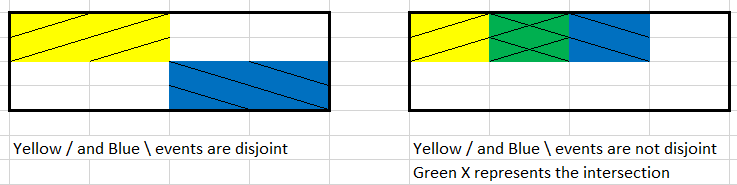
\includegraphics[width=10.24in]{_graphics/venn-disjoint} \caption{Illustration of countable additivity for two events. The events in the picture on the left are disjoint, but not on the right.}\label{fig:venn-disjoint}
\end{figure}

In Example \ref{exm:worldseries}, the events \(A\)=``the Astros win the 2019 World Series'' and \(D\)=``the Dodgers win the 2019 World Series'' are disjoint \(A\cap D = \emptyset\); in a single World Series, both teams cannot win. Therefore, the probability of \(A\cup D\), the event that either the Astros or the Dodgers win, must be 46\%.

The three axioms of a probability measure are minimal logical consistency requirements that must be satisfied by any probability model. There are also many physical aspects of the random phenomenon or assumptions (e.g.
``fairness'', independence, conditional relationships) that must be considered when determining a reasonable
probability measure for a particular situation. Often, \(\IP\) is defined implicitly through modeling
assumptions, and probabilities of events follow from the
axioms and related properties.

Many other properties follow from the axioms. The main ``meat'' of the axioms is countable additivity. Thus, the key to many proofs of probability properties is to write relevant events in terms of disjoint events.

\begin{theorem}[Properties of a probability measure.]
\protect\hypertarget{thm:prob-properties}{}{\label{thm:prob-properties} \iffalse (Properties of a probability measure.) \fi{} }
Complement rule\footnote{Proof: Since \(\Omega = A \cup A^c\) and \(A\) and \(A^c\) are disjoint the axioms imply that \(1=\IP(\Omega) = \IP(A \cup A^c) = \IP(A) + \IP(A^c)\).}. For any event \(A\), \(\IP(A^c) = 1 - \IP(A)\). In particular, since \(\Omega^c=\emptyset\), \(\IP(\emptyset)=0\).

Subset rule\footnote{Proof. If \(A \subseteq B\) then \(B = A \cup (B \cap A^c)\). Since \(A\) and \((B \cap A^c)\) are disjoint, \(\IP(B) = \IP(A) + \IP(B \cap A^c) \ge \IP(A)\).}. If \(A \subseteq B\) then \(\IP(A) \le \IP(B)\).

General addition rule for two events\footnote{The proof is easiest to see by considering a picture like the one Figure \ref{fig:venn-disjoint} .}. If \(A\) and \(B\) are any two events
\begin{align*}
\IP(A\cup B) = \IP(A) + \IP(B) - \IP(A \cap B)
\end{align*}

Law of total probability. If \(B_1,\ldots, B_k\) are disjoint with \(B_1\cup \cdots \cup B_k=\Omega\), then
\begin{align*}
\IP(A) & = \sum_{i=1}^k \IP(A \cap B_i)
\end{align*}
\end{theorem}

The key to the proofs is to represent relevant events in terms of disjoint events and use countable addivity (and the other axioms).

Note: \(A\cup B\) is inclusive so we \emph{do} want to count the possibility of both, \(A\cap B\). The problem with simply adding \(\IP(A)\) and \(\IP(B)\) is that their sum \emph{double counts} \(A \cap B\). We do want to count the outcomes that satisfy both \(A\) and \(B\), but we only want to count them once. Subtracting \(\IP(A \cap B)\) in the general addition rule for two events corrects for the double counting.

For example, consider the picture on the right in Figure \ref{fig:venn-disjoint}. Suppose each rectangular cell represents a distinct outcome; there are 16 outcomes in total. Assume the outcomes are equally likely, each with probability \(1/16\). Let \(A\) represent the yellow / event which has probability \(4/16\) and let \(B\) represent the blue \textbackslash{} event which has probability 4/16. Then \(\IP(A\cup B) = 6/16\), since there are 6 outcomes which satisfy either event \(A\) or \(B\) (or both). However, simply adding \(\IP(A)+\IP(B)\) yields \(8/16\) because the two outcomes that satisfy the green event \(A\cap B\) are counted both in \(\IP(A)\) and \(\IP(B)\). So to correct for this double counting, we subtract out \(\IP(A\cap B)\):
\[
\IP(A)+\IP(B)-\IP(A\cap B) = 4/16 + 4/16 -2/16 = 6/16 = \IP(A\cup B)
\]

Warning: The general addition rule for more than two events is more complicated\footnote{For three events, \(\IP(A\cup B\cup C) = \IP(A) + \IP(B) + \IP(C) - \IP(A\cap B) - \IP(A \cap C) - \IP(B \cap C) + \IP(A \cap B \cap C)\).}; see \href{https://en.wikipedia.org/wiki/Inclusion\%E2\%80\%93exclusion_principle\#In_probability}{the inclusion-exclusion principle}.

In the law of total probability\footnote{We will see a different expression of the law of total probability, involving conditional probabilities, in Section \ref{lawtotalprob}.} the events \(B_1, \ldots, B_k\), which represent ``cases'', form a \emph{partition} of the sample space; each outcome \(\omega\in\Omega\) lies in exactly one of the \(B_i\). The law of total probability says that we can interpret the ``overall'' probability \(\IP(A)\) by summing the probability of \(A\) in each ``case'' \(\IP(A\cap B_i)\).

\begin{exercise}
\protect\hypertarget{exr:linda}{}{\label{exr:linda} }Consider a Cal Poly student who frequently has blurry, bloodshot eyes, generally exhibits slow reaction time, always seems to have the munchies, and disappears at 4:20 each day. Which of the following events, \(A\) or \(B\), has a higher probability? (Assume the two probabilities are not equal.)

\begin{itemize}
\tightlist
\item
  \(A\): The student has a GPA above 3.0.
\item
  \(B\): The student has a GPA above 3.0 and smokes marijuana regularly.
\end{itemize}
\end{exercise}

\textbf{Warning!} Your psychological judgment of probabilities is often inconsistent with the mathematical logic of probabilities.

\begin{example}[Don't do what Donny Don't does.]
\protect\hypertarget{exm:dd-notation}{}{\label{exm:dd-notation} \iffalse (Don't do what Donny Don't does.) \fi{} }
At various points in his homework, Donny Don't writes the following. Explain to Donny, both mathematically and intuitively, why each of the following symbols is nonsense. Below, \(A\) and \(B\) represent events, \(X\) and \(Y\) represent random variables.
\end{example}

\begin{enumerate}
\def\labelenumi{\arabic{enumi}.}
\tightlist
\item
  \(\IP(A = 0.5)\)
\item
  \(\IP(A + B)\)
\item
  \(\IP(A) \cup \IP(B)\)
\item
  \(\IP(X)\)
\item
  \(\IP(X = A)\)
\item
  \(\IP(X \cap Y)\)
\end{enumerate}

\begin{solution}
\iffalse{} {Solution. } \fi{}to Example \ref{exm:dd-notation}
\end{solution}

\begin{enumerate}
\def\labelenumi{\arabic{enumi}.}
\tightlist
\item
  \(A\) is a set and 0.5 is a number; it doesn't make mathematical sense to equate them. Suppose that \(A\) is the event that is rains tomorrow. It doesn't make sense to say (as \(A=1\) does) ``it rains tomorrow equals 0.5''. If we want to say ``the probability that it rains tomorrow equals 0.5'' we should write \(\IP(A) = 0.5\).
\item
  \(A\) and \(B\) are sets; it doesn't make mathematical sense to add them. Suppose that \(B\) is the event that tomorrow's high temperature is above 80 degrees F. It doesn't make sense to say (as \(A+B\) does) ``the sum of (it rains tomorrow) and (tomorrow's high temperature is above 80 degrees F)''. If we want ``(it rains tomorrow) OR (tomorrow's high temperature is above 80 degrees F)'', then we need \(A\cup B\). Union is an operation on sets; addition is an operation on numbers.
\item
  \(\IP(A)\) and \(\IP(B)\) are numbers; union is an operation on sets, it doesn't make mathematical sense to take a union of numbers. Since \(\IP(A)\) and \(\IP(B)\) are numbers then mathematically we can add them. But keep in mind that \(\IP(A)+\IP(B)\) is not necessarily a probability, for example if \(\IP(A)=0.5\) and \(\IP(B)=0.6\). If we want ``the probability that (it rains tomorrow) OR (tomorrow's high temperature is above 80 degrees F)'' then the correct symbol is \(\IP(A\cup B)\), which would be equal to \(\IP(A)+\IP(B)\) only if \(A\) and \(B\) were disjoint (which in the example would mean it's not possible to have a rainy day with a high temperature above 80 degrees F).
\item
  \(X\) is a random variable, and probabilities are assigned to events. If \(X\) is tomorrow's high temperature in degrees F then \(P(X)\) reads ``the probability that tomorrow's high temperature in degrees F'', which is missing any qualifying information that could define an event. We could write \(\IP(X>80)\) to represent ``the probability that (tomorrow's high temperature is greater than 80 degrees F)''.
\item
  \(X\) is a random variable (a function) and \(A\) is an event (a set), and it doesn't make sense to equate these two different mathematical objects. It doesn't make sense to say (as \(X=A\) does) ``tomorrow's high temperature in degrees F equals the event that it rains tomorrow''.
\item
  \(X\) and \(Y\) are RVs (functions) and intersection is an operation on sets. If \(Y\) is the amount of rainfall in inches tomorrow then \(X \cap Y\) is attempting to say ``tomorrow's high temperature in degrees F and the amount of rainfall in inches tomorrow'', but this is still missing qualifying information to define a valid event for which a probability can be assigned. We could say \(\IP(\{X > 80\} \cap \{Y < 2\})\) to represent ``the probability that (tomorrow's high temperature is greater than 80 degrees F) AND (the amount of rainfall tomorrow is less than 2 inches)''.
\end{enumerate}

\hypertarget{probability-measures-in-a-dice-rolling-example}{%
\subsection{Probability measures in a dice rolling example}\label{probability-measures-in-a-dice-rolling-example}}

A probability measure is a \emph{set function}: \(\IP:\mathcal{F}\mapsto[0, 1]\) takes as an input an event (set) \(A\in\mathcal{F}\) and returns as an output a number \(\IP(A)\in[0,1]\). Sometimes \(\IP(A)\) is defined explicitly for an event \(A\) via a formula.

As an example, consider a single roll of a four-sided die. The sample space consists of the four possible outcomes \(\Omega = \{1, 2, 3, 4\}\). Let's first assume that the die is fair, so all four outcomes are equally likely, each with probability\footnote{That the probability of each outcome must be 1/4 when there are four \emph{equally likely} outcomes follows from the axioms, by writing \(\{1, 2, 3, 4\} = \{1\}\cup\{2\}\cup \{3\}\cup \{4\}\), a union of disjoint sets, and applying countable additivity and \(\IP(\Omega)=1\).} 1/4. Given that the probability of each outcome\footnote{A probability measure is always defined on sets. When we say loosely "the probability of an outcome \(\omega\)'\,' we really mean the probability of the event consisting of the single outcome \(\{\omega\}\). In this example \(\IP(\{\omega\})=1/4\) for \(\omega\in\{1, 2, 3, 4\}\)} is 1/4, countable additivity implies

\[
\IP(A) = \frac{\text{number of elements in $A$}}{4}, \qquad{\text{$\IP$ assumes a fair four-sided die}}
\]

The following table lists all the possible events, and their probability under the assumption of equally likely outcomes.

\begin{longtable}[]{@{}lll@{}}
\caption{\label{tab:die-events-fair} All possible events associated with a single roll of a four-sided die, and their probabilities assuming the die is fair.}\tabularnewline
\toprule
Event & Description & Probability of event assuming equally likely outcomes\tabularnewline
\midrule
\endfirsthead
\toprule
Event & Description & Probability of event assuming equally likely outcomes\tabularnewline
\midrule
\endhead
\(\emptyset\) & Roll nothing (not possible) & 0\tabularnewline
\(\{1\}\) & Roll a 1 & 1/4\tabularnewline
\(\{2\}\) & Roll a 2 & 1/4\tabularnewline
\(\{3\}\) & Roll a 3 & 1/4\tabularnewline
\(\{4\}\) & Roll a 4 & 1/4\tabularnewline
\(\{1, 2\}\) & Roll a 1 or a 2 & 2/4\tabularnewline
\(\{1, 3\}\) & Roll a 1 or a 3 & 2/4\tabularnewline
\(\{1, 4\}\) & Roll a 1 or a 4 & 2/4\tabularnewline
\(\{2, 3\}\) & Roll a 2 or a 3 & 2/4\tabularnewline
\(\{2, 4\}\) & Roll a 2 or a 4 & 2/4\tabularnewline
\(\{3, 4\}\) & Roll a 3 or a 4 & 2/4\tabularnewline
\(\{1, 2, 3\}\) & Roll a 1, 2, or 3 (a.k.a. do not roll a 4) & 3/4\tabularnewline
\(\{1, 2, 4\}\) & Roll a 1, 2, or 4 (a.k.a. do not roll a 3) & 3/4\tabularnewline
\(\{1, 3, 4\}\) & Roll a 1, 3, or 4 (a.k.a. do not roll a 2) & 3/4\tabularnewline
\(\{2, 3, 4\}\) & Roll a 2, 3, or 4 (a.k.a. do not roll a 1) & 3/4\tabularnewline
\(\{1, 2, 3, 4\}\) & Roll something & 1\tabularnewline
\bottomrule
\end{longtable}

The above assignment satsifies all the axioms and so it represents a valid probability measure. But assuming that the outcomes are equally likely requires much more than the basic logical consistency requirements of the axioms. There are many other possible probability measures, like in the following.

\begin{example}
\protect\hypertarget{exm:die-weighted}{}{\label{exm:die-weighted} }Now consider a single roll of a four-sided die, but suppose the die is weighted so that the outcomes are no longer equally likely (but each outcome is still possible). Suppose that the probability of event \(\{2, 3\}\) is 0.5, of event \(\{3, 4\}\) is 0.7, and of event \(\{1, 2, 3\}\) is 0.6. Complete a table, like the one for the equally likely outcome scenario above, listing the probability of each event for this particular weighted die. In what particular way is the die weighted? That is, what is the probability of each the four possible outcomes?
\end{example}

\begin{solution}
\iffalse{} {Solution. } \fi{}to Example \ref{exm:die-weighted}
\end{solution}

Since the probability of not rolling a 4 is 0.6, the probability of rolling a 4 must be 0.4. Since \(\{3, 4\} = \{3\} \cup \{4\}\), a union of disjoint sets, the probability of rolling a 3 must be 0.3. Similarly, the probability of rolling a 2 must be 0.2, and the probability of rolling a 1 must be 0.1. The table below list the probabilities of the possible events for this particular weighted die.

\begin{longtable}[]{@{}lll@{}}
\caption{\label{tab:die-events-weighted} All possible events associated with a single roll of a fair-sided die, and their probabilities assuming the die is weighted: roll a 1 with probability 1/10, 2 with probability 2/10, 3 with probability 3/10, 4 with probability 4/10.}\tabularnewline
\toprule
Event & Description & Probability of event assuming a particular weighted die\tabularnewline
\midrule
\endfirsthead
\toprule
Event & Description & Probability of event assuming a particular weighted die\tabularnewline
\midrule
\endhead
\(\emptyset\) & Roll nothing (not possible) & 0\tabularnewline
\(\{1\}\) & Roll a 1 & 0.1\tabularnewline
\(\{2\}\) & Roll a 2 & 0.2\tabularnewline
\(\{3\}\) & Roll a 3 & 0.3\tabularnewline
\(\{4\}\) & Roll a 4 & 0.4\tabularnewline
\(\{1, 2\}\) & Roll a 1 or a 2 & 0.3\tabularnewline
\(\{1, 3\}\) & Roll a 1 or a 3 & 0.4\tabularnewline
\(\{1, 4\}\) & Roll a 1 or a 4 & 0.5\tabularnewline
\(\{2, 3\}\) & Roll a 2 or a 3 & 0.5\tabularnewline
\(\{2, 4\}\) & Roll a 2 or a 4 & 0.6\tabularnewline
\(\{3, 4\}\) & Roll a 3 or a 4 & 0.7\tabularnewline
\(\{1, 2, 3\}\) & Roll a 1, 2, or 3 (a.k.a. do not roll a 4) & 0.6\tabularnewline
\(\{1, 2, 4\}\) & Roll a 1, 2, or 4 (a.k.a. do not roll a 3) & 0.7\tabularnewline
\(\{1, 3, 4\}\) & Roll a 1, 3, or 4 (a.k.a. do not roll a 2) & 0.8\tabularnewline
\(\{2, 3, 4\}\) & Roll a 2, 3, or 4 (a.k.a. do not roll a 1) & 0.9\tabularnewline
\(\{1, 2, 3, 4\}\) & Roll something & 1\tabularnewline
\bottomrule
\end{longtable}

The symbol \(\IP\) is more than just shorthand for the word ``probability''. \(\IP\) denotes the underlying probability measure, which represents all the assumptions about the probability model. Changing assumptions results in a change of the probability measure. We often consider several probability measures for the same sample space and collection of events; these several measures represent different sets of assumptions and different probability models.

In the dice example above, suppose \(\IP\) represents the probability measure corresponding to the assumption of a fair die (equally likely outcomes). With this measure \(\IP(A) = 2/4\) for \(A = \{1, 2\}\). Now let \(\IQ\) represent the probability measure corresponding to the assumption of the weighted die; then \(\IQ(A) = 0.3\). The outcomes and events are the same in both scenarios, because both scenarios involve a four sided-die. What is different is the probability measure that assigns probabilities to the events. One scenario assumes the die is fair while the other assumes the die has a particular weighting, resulting in two different probability measures.

Both probability measures in the dice example could be written as explicit set functions: for an event \(A\)

\begin{align*}
\IP(A) & = \frac{\text{number of elements in $A$}}{4}, & & {\text{$\IP$ assumes a fair four-sided die}}
\\
\IQ(A) & = \frac{\text{sum of elements in $A$}}{10}, & & {\text{$\IQ$ assumes a particular weighted four-sided die}}
\end{align*}

We provide the above descriptions to illustrate that a probability measure operates on sets. However, in many situations there does not exist a simple closed form expression for the set function defining the probability measure which maps events to probabilities.

Perhaps the concept of multiple potential probability measures is easier to understand in a subjective probability situation. For example, each model that is used to forecast the 2019 NFL season corresponds to a probability measure which assigns probabilities to events like ``the Eagles win the 2019 Superbowl''. Different sets of assumptions and models can assign different probabilities for the same events.

\begin{itemize}
\tightlist
\item
  A single probability measure corresponds to a particular set of assumptions about the random phenomenon.
\item
  There can be many probability measures defined on a single sample space, each one corresponding to a different probabilistic model.
\item
  Probabilities of events can change if the probability measure changes.
\end{itemize}

\hypertarget{uniform-probability-measures-sec-uniform-prob}{%
\subsection{Uniform probability measures \#\{sec-uniform-prob\}}\label{uniform-probability-measures-sec-uniform-prob}}

Sometimes \(\IP(A)\) is defined explicitly for an event \(A\) via a formula. For example, in the case of a finite sample space with \textbf{equally likely outcomes},

\[
\IP(A) = \frac{|A|}{|\Omega|} = \frac{\text{number of outcomes in $A$}}{\text{number of outcomes in $\Omega$}} \qquad{\text{when outcomes are equally likely}}
\]

\begin{example}
\protect\hypertarget{exm:coin-probspace}{}{\label{exm:coin-probspace} }
Flip a coin 4 times, and record the result of each trial in sequence. For example, HTTH means heads on the first on last trial and tails on the second and third. The sample space consists of 16 possible outcomes. One choice of probability measure \(\IP\) corresponds to assuming the 16 possible outcomes are equally likely. (This assumes that the coin is fair and the flips are independent.)
\end{example}

\begin{enumerate}
\def\labelenumi{\arabic{enumi}.}
\tightlist
\item
  Specify the probability of each individual outcome, e.g.~\(\{HHTH\}\).\\
\item
  Find \(\IP(A)\), where \(A\) is the event that exactly 3 of the flips land on heads.
\item
  Find \(\IP(B)\), where \(B\) is the event that exactly 4 of the flips land on heads.
\item
  Find and interpret \(\IP(A \cup B)\).
\item
  Find \(\IP(E_1)\), the event that the first flip results in heads.
\item
  Find \(\IP(E_2)\), the event that the second flip results in heads.
\item
  Find and interpret \(\IP(E_1 \cup E_2)\).
\item
  We assumed the 16 outcomes are equally likely. Do the axioms require this assumption?
\end{enumerate}

\begin{solution}
\iffalse{} {Solution. } \fi{}
to Example \ref{exm:coin-probspace}
\end{solution}

\begin{enumerate}
\def\labelenumi{\arabic{enumi}.}
\tightlist
\item
  The sample space is composed of 16 outcomes which are assumed to be equally likely, so the probability of each outcome is 1/16.
\item
  \(A = \{HHHT, HHTH, HTHH, THHH\}\) is the event that exactly 3 of the flips land on heads. Since \(A\) consists of 4 distinct equally likely outcomes, \(\IP(A) = 4/16\).
\item
  \(B = \{HHHH\}\), av event consisting of a single outcome, so \(\IP(B) = 1/16\).
\item
  Directly, \(A \cup B = \{HHHT, HHTH, HTHH, THHH, HHHH\}\), so \(\IP(A\cup B) = 5/16\). Also \(A\) and \(B\) are disjoint, so \(\IP(A \cup B) = \IP(A) + \IP(B) = 4/16 + 1/16 = 5/16\).
\item
  Intuitively this is 1/2, but sample space outcomes consist of a sequence of four coin flips, so we should define the proper event.
  \[
  E_1 = \{HHHH, HHHT, HHTH, HTHH, HHTT, HTHT, HTTH, HTTT\}
  \]
  So \(\IP(E_1) = 8/16 = 1/2\).
\item
  Similar to the previous part.
  \[
  E_2 = \{HHHH, HHHT, HHTH, THHH, HHTT, THHT, THTH, THTT\}
  \]
  So \(\IP(E_2) = 8/16 = 1/2\).
\item
  \(E_1 \cup E_2\) is the event that at least one of the first two flips is heads:
  \begin{align*}
  E_1 \cup E_2 & = \{HHHH, HHHT, HHTH, HTHH, THHH, HHTT,
  \\
  & \quad HTHT, HTTH, THHT, THTH, HTTT, THTT\}
  \end{align*}
  So \(\IP(E_1 \cup E_2) = 12/16\). Note that \(\E_1\) and \(\E_2\) are not disjoint, so we cannot just add their probabilities. But we can use the general addition rule for two events.
  \[
  E_1 \cap E_2 = \{HHHH, HHHT, HHTH, HHTT\}
  \]
  So \(\IP(E_1 \cup E_2) = \IP(E_1) + \IP(E_2) - \IP(E_1 \cap E_2) = 8/16 + 8/16 - 4/16 = 12/16\).
\item
  No, the axioms do not require equally likely outcomes. If, for example, the coin were biased in favor of landing on Heads, we would want a different probability measure.
\end{enumerate}

Probabilities are always defined for events (sets) but to shorten notation, it is common to write \(\IP(X=3)\) instead of \(\IP(\{X=3\})\), and \(\IP(X = 4, Y = 3)\) instead of \(\IP(\{X = 4\}\cap \{Y = 3\})\). But keep in mind that an expression like ``\(X=3\)'' really represents an event \(\{X=3\}\), an expression which itself represents \(\{\omega\in\Omega: X(\omega) = 3\}\), a subset of \(\Omega\).

Probabilities involving multiple events, such as \(\IP(A \cap B)\) or \(\IP(X=4, Y=3)\), are often called \textbf{joint probabilities}.

\begin{example}
\protect\hypertarget{exm:dice-probspace}{}{\label{exm:dice-probspace} }
Roll a four-sided die twice, and record the result of each roll in sequence. For example, the outcome \((3, 1)\) represents a 3 on the first roll and a 1 on the second; this is not the same outcome as \((1, 3)\). One choice of probability measure corresponds to assuming that the die is fair and that the 16 possible outcomes are equally likely. Let \(X\) be the sum of the two dice, and let \(Y\) be the larger of the two rolls (or the common value if both rolls are the same).
\end{example}

\begin{enumerate}
\def\labelenumi{\arabic{enumi}.}
\tightlist
\item
  Find the probability of each individual outcome, e.g., \(\{(3, 1)\}\).
\item
  Find \(\IP(A)\) where \(A\) is the event the the sum of the dice is 4.
\item
  Find \(\IP(B)\) where \(B\) is the event the the sum of the dice is at most 3.
\item
  Find \(\IP(\{Y = 3\})\) a.k.a. \(\IP(Y=3)\).
\item
  Find \(\IP(\{Y \le 3\})\) a.k.a. \(\IP( Y\le 3)\).
\item
  Find \(\IP(\{X = 4\}\cap \{Y = 3\})\) a.k.a. \(\IP(X=4, Y=3)\) a.k.a. \(\IP(\{(X,Y) = (4,3)\})\).
\item
  Are the values of \(X\) equally likely? The values of \(Y\)? The values of \((X, Y)\)?
\end{enumerate}

\begin{solution}
\iffalse{} {Solution. } \fi{}
to Example \ref{exm:dice-probspace}
\end{solution}

\begin{enumerate}
\def\labelenumi{\arabic{enumi}.}
\tightlist
\item
  Since 16 distinct, equally likely outcomes comprise the total probability of 1, the probability of each individual outcome must be 1/16.
\item
  The event that the sum of the dice is 4 is \(A = \{(1, 3), (2, 2), (3, 1)\}\) which can be written as a union of three disjoint sets \(A = \{(1, 3)\} \cup \{(2, 2)\} \cup \{(3, 1)\}\). Therefore, \(\IP(A) = \IP(\{(1, 3)\}) + \IP(\{(2, 2)\}) + \IP(\{(3, 1)\}) = 1/16 + 1/16 + 1/16 = 3/16 = 0.1875\).
\item
  The event the the sum of the dice is at most 3 is \(B=\{(1, 1), (1, 2), (2, 1)\}\), and so similarly to the previous part, \(\IP(B) = 3/16=0.1875\).
\item
  Remember that \(\{Y=3\}\) represents the event that that larger of the two rolls is 3, \(\{Y=3\}=\{(1, 3), (2, 3), (3, 3), (3, 1), (3, 2)\}\), an event which can be written as the union of 5 disjoint events each having probability 1/16. Then \(\IP(\{Y = 3\}) = 5/16=0.3125\).
\item
  \(\{Y \le 3\}=\{(1, 1), (1, 2), (1, 3), (2, 1), (2, 2), (2, 3), (3, 1), (3, 2), (3, 3)\}\) so similar to the previous parts \(\IP(Y \le 3) = 9/16=0.5625\).
\item
  \(\{X = 4\}\cap \{Y = 3\} = \{(3, 1), (1, 3)\}\) so \(\IP(\{X = 4\}\cap \{Y = 3\})= 2/16 = 0.125\)
\item
  The values of \(X\) are not equally likely; for example, \(\IP(\{X=4\}) = 3/16\) but \(\IP(\{X=2\})=\IP\{(1, 1)\} = 1/16\). The values of \(Y\) are also not equally likely; for example, \(\IP(\{Y=3\})=5/16\) but \(\IP(\{Y=1\})= \IP\{(1, 1)\} = 1/16\). And the values of \((X, Y)\) pairs are also not equally likely; for example, \(\IP(\{(X, Y) = (4, 3)\}) = 2/16\) but \(\IP(\{(X,Y) = (1, 1)\}) = 1/16\). So just because the underlying outcomes of the sample space are equally likely does not necessarily imply that everything of interest is equally likely as well.
\end{enumerate}

\begin{example}[Matching problem]
\protect\hypertarget{exm:matching-probspace}{}{\label{exm:matching-probspace} \iffalse (Matching problem) \fi{} }Recall the ``matching problem''.
A set of \(n\) cards labeled \(1, 2, \ldots, n\) are placed in \(n\)
boxes labeled \(1, 2, \ldots, n\), with exactly one card in each box.
Consider the case \(n=4\). Let
\(Y\) be the number of cards (out of 4) which match the number of the
box in which they are placed.

We can consider as the sample space the possible ways in which the cards can be distributed to the four boxes. For example, 3214 represents that card 3 is returned (wrongly) to the first box, card 2 is returned (correctly) to the second box, etc. So the sample space consists of the following 24 outcomes\footnote{There are 4 cards that could potentially go in box 1, then 3 cards that could potentially go in box 2, 2 in box 3, and 1 left for box 4. This results in \(4\times3\times2\times1=4! = 24\) possible outcomes.}, which we will assume are equally likely.

\begin{center}\rule{0.5\linewidth}{0.5pt}\end{center}

\begin{verbatim}
1234   1243   1324   1342   1423   1432   2134   2143
2314   2341   2413   2431   3124   3142   3214   3241
3412   3421   4123   4132   4213   4231   4312   4321
                                               
\end{verbatim}

\begin{center}\rule{0.5\linewidth}{0.5pt}\end{center}
\end{example}

\begin{enumerate}
\def\labelenumi{\arabic{enumi}.}
\tightlist
\item
  What are the possible values of \(Y\)? Find \(\IP(Y=y)\) for each possible value of \(y\).
\item
  Let \(B\) be the event that at least one card is placed in the correct box. Find \(\IP(B)\).
\item
  Let \(B_1\) be the event that card 1 is placed in box 1, and define \(B_2, B_3, B_4\) similarly. Represent the event \(B\) in terms of \(B_1, B_2, B_3, B_4\).
\item
  Find \(\IP(B_1)\). Also find \(\IP(B_2)\), \(\IP(B_3)\), \(\IP(B_4)\).
\item
  Find \(\IP(B_1\cap B_2 \cap B_3 \cap B_4)\).
\item
  Is it possible to compute \(\IP(B_1 \cup B_2 \cup B_3 \cup B_4)\) based on just the five probabilities from the previous two parts?
\end{enumerate}

\begin{solution}
\iffalse{} {Solution. } \fi{}
to Example \ref{exm:matching-probspace}
\end{solution}

The following table evaluates \(Y\) for each of the possible outcomes.

\begin{center}\rule{0.5\linewidth}{0.5pt}\end{center}

\begin{verbatim}
Y(1234)=4   Y(1243)=2   Y(1324)=2   Y(1342)=1   Y(1423)=1   Y(1432)=2   Y(2134)=2   Y(2143)=0
Y(2314)=1   Y(2341)=0   Y(2413)=0   Y(2431)=1   Y(3124)=1   Y(3142)=0   Y(3214)=2   Y(3241)=1
Y(3412)=0   Y(3421)=0   Y(4123)=0   Y(4132)=1   Y(4213)=1   Y(4231)=2   Y(4312)=0   Y(4321)=0
                                               
\end{verbatim}

\begin{center}\rule{0.5\linewidth}{0.5pt}\end{center}

\begin{enumerate}
\def\labelenumi{\arabic{enumi}.}
\tightlist
\item
  The possible values of \(Y\) are 0, 1, 2, 4. \(Y\) cannot be 3, since if 3 cards match, then the fourth card must necessarily match too. \(\IP(Y=0)=9/24\), \(\IP(Y=1)=8/24\), \(\IP(Y=2)=6/24\), \(\IP(Y=4)=1/24\).
\item
  \(\IP(B) = \IP(Y\ge 1) = 1 - \IP(Y=0) = 15/24 = 0.625\).
\item
  \(B = B_1\cup B_2\cup B_3\cup B_4\).
\item
  Intuitively, \(\IP(B_1)=1/4\) since card 1 is equally likely to be placed in any of the 4 boxes. In terms of the sample space outcomes, \(B_1 =\{1234, 1234, 1243, 1324, 1342, 1423, 1432\}\), so \(\IP(B_1)=6/24=1/4\). Also \(\IP(B_2)=\IP(B_3)=\IP(B_4)=6/24\).
\item
  \(\IP(B_1\cap B_2 \cap B_3 \cap B_4) = \IP({1234}) = 1/24\).
\item
  Nope. The events are not disjoint, so you can't just add their probabilities. Also note that \(\IP(B_1\cup B_2 \cup B_3\cup B_4)\neq \IP(B_1)+\IP(B_2)+\IP(B_3)+\IP(B_4)-\IP(B_1\cap B_2 \cap B_3 \cap B_4)\). As we mentioned previously, the general addition rule is complicated for more than two events.
\end{enumerate}

For finite sample spaces with equally likely outcomes, computing the probability of an event reduces to counting the number of outcomes that satisfy the event. The continuous analog of equally likely outcomes is a \textbf{uniform probability measure}. When the sample space is uncountable, size is measured continuously (length, area, volume) rather that discretely (counting).

\[
\IP(A) = \frac{|A|}{|\Omega|} = \frac{\text{size of } A}{\text{size of } \Omega} \qquad \text{for a uniform probability measure $\IP$}
\]

\begin{example}
\protect\hypertarget{exm:uniform-probspace}{}{\label{exm:uniform-probspace} }
Suppose the spinner in Figure \ref{fig:uniform-spinner} is spun twice. Let the sample space be \(\Omega = [0,1]\times [0,1]\) and let \(\IP\) be the uniform probability measure. Find the probability of each of the following events. (Hint: recall that these events are depicted in Figure \ref{fig:uniform-event-plot})
\end{example}

\begin{enumerate}
\def\labelenumi{\arabic{enumi}.}
\tightlist
\item
  \(A\), the event that the first spin is larger then the second.
\item
  \(B\), the event that the smaller of the two spins (or common value if a tie) is less than 0.5.
\item
  \(C\), the event that the sum of the two dice is less than 1.5.
\item
  \(D\), the event that the first spin is less than 0.4.
\end{enumerate}

\begin{solution}
\iffalse{} {Solution. } \fi{}
to Example \ref{exm:uniform-probspace}
\end{solution}

\begin{enumerate}
\def\labelenumi{\arabic{enumi}.}
\tightlist
\item
  \(\IP(A) = 0.5\). The shaded triangle makes up half the area of the square. This should make sense because the first spin should be equally likely to be the larger of the two spins.\\
\item
  \(\IP(B) = 0.75\).
\item
  \(\IP(C)=0.875\). The unshaded triangle, representing \(C^c\), has area \((1/2)(0.5)(0.5) = 0.125\).
\item
  \(\IP(D) = 0.4.\)
\end{enumerate}

ADD plots of shaded rectangles

\hypertarget{non-uniform-probability-measures}{%
\subsection{Non-uniform probability measures}\label{non-uniform-probability-measures}}

For countable sample spaces, the probability measure is often defined by specifying the probability of each individual outcome. Then the probability of an event is obtained by summing the probabilities of the outcomes which comprise the event. Such was the case in Example \ref{exm:die-weighted}; we could have specified the probability measuring by providing the probability of each face (1 with probability 0.1, \ldots, 4 with probability 0.4) and then obtained probabilities of all the events in Table \ref{tab:die-events-weighted} by adding the appropriate outcome probabilities.

For uncountable sample spaces, integration typically plays the analogous role that summation plays for countable sample spaces.

\begin{example}
\protect\hypertarget{exm:exponential-probspace}{}{\label{exm:exponential-probspace} }Consider the sample space \(\Omega=[0,\infty)\) with a probability measure\footnote{This defines the Exponential(1) distribution; see Section \ref{exponential}.} defined by
\[
  \IP(A) = \int_A e^{-u}\, du, \qquad A \subseteq [0, \infty).
\]
\end{example}

\begin{enumerate}
\def\labelenumi{\arabic{enumi}.}
\tightlist
\item
  Verify that \(\IP(\Omega)=1\).
\item
  Compute \(\IP(A)\) for \(A=[0, 1]\).
\item
  Without integrating again, compute \(\IP(B)\) for \(B=(1, \infty)\).
\item
  Compute \(\IP(C)\) for \(C=[0, 1] \cup (2, 4)\).
\end{enumerate}

\begin{solution}
\iffalse{} {Solution. } \fi{}to Example \ref{exm:exponential-probspace}
\end{solution}

  \bibliography{book.bib,packages.bib}

\end{document}
